\chapter{Verification and Validation}
 Computer simulations are in many engineering applications a cost-efficient method of conducting design and optimize performance. However, blindly trusting results generated from a computer simulations can prove to be naive. It doesn't take a lot of coding experience before one realizes many things that can brake down and produce unwanted or unexpected results. 
Therefore, \textit{credibility} of computational results are essential, meaning the simulation is worthy of belief or confidence \cite{Oberkampf2010}. For rigid evaluation of numerical models we use \textit{verification and validation} ($V\&V$) \cite{Sommerville2006}. For a in-depth discussion of all aspects surrounding $V\&V$ the reader is referred to \cite{Oberkampf2010}. In this thesis, we follow the definitions provided by the \textit{American Society of Mechanical Engineers guide for Verification and Validation in Computational Solid Mechanics}  \cite{Schwer2006}:
\begin{defn}
Verification: The process of determining that a computational model accurately represents
the underlying mathematical model and its solution. 
\end{defn}
\begin{defn}
Validation: The process of determining the degree to which a model is an accurate
representation of the real world from the perspective of the intended uses of the model. 
\label{eq:intcond}
\end{defn}
Simplified, \textit{verification} considers if one solves the equations right, while \textit{validation} is checking if one solves the right equations for the given problem \cite{Roache}. Verification and validation is per definition an ongoing processes, with no clear boundary of completeness unless additional requirements are specified \cite{Roache}. The goal of this chapter is to verify the implementations using the method of manufactured solution (MMS), and addressing validation in a subsequent chapter.
\section{Verification of Code}
Within scientific computing a mathematical model is often the baseline for simulations of a particular problem of interest. For scientists exploring physical phenomena, the mathematical model is often on the form of systems of partial differential equations (PDEs). Through verification of code, the ultimate goal is to ensure that the computer program correctly represents the mathematical model. To accumulate sufficient evidence that a mathematical model is solved correctly by a computer code, it must excel within predefined criteria. If the acceptance criterion is not satisfied, a coding mistake is suspected. Should the code pass the preset criteria, the code is considered verified. Of the different classes of test found in \cite{Roache},  \textit{order-of-accuracy} is regarded as the most rigorous  \cite{Biggs, Roache, Etienne2006}. The method tests if the discretization error $E$ is reduced in accordance with the \textit{formal order of accuracy} expected from the numerical scheme. The formal order of accuracy is defined to be the theoretical rate at which the truncation error of a numerical scheme is expected to reduce. The \textit{observed order of accuracy} is the actual rate produced by the numerical solution.
For order of convergence tests, the code is assumed to be verified if we recover the theoretical convergence from the discretization error. Monitoring the discretization error $E$ by spatial and temporal refinements, one assumes the error $E$ can be expressed as,
\begin{align*}
&E = C\Delta t^p + D\Delta x^l\\
\end{align*} 
where C and D are constants, $\Delta t$ and $\Delta x$ represents the spatial and temporal resolution, while $p$ and $l$ is the observed order of accuracy of the numerical scheme. 
In order to calculate the convergence in space $l$, the spatial discretization error must be negligible compared to the temporal discretization error $C\Delta t^p$. The total error can then by expressed as $E =  D\Delta x^l$, and we calculate the convergence rate for subsequent spatial mesh refinement by,
\begin{align}
\frac{E_2}{E_1} = (\frac{\Delta x_2}{\Delta x_1})^l \\
l = \frac{log (\frac{E_2}{E_1})}{ log (\frac{\Delta x_2}{\Delta x_1}) }
\end{align}
where $E_2$ is computed on a finer mesh compared to $E_1$ on a courser mesh. For spatial convergence tests, the same procedure applies by choosing a high resolution temporal discretization, and calculating the error $E_1$,$E_2$ by subsequent smaller time steps. In order to calculate order of convergence we need to find an exact solution of the problem. Creating an exact solution is often non-trivial. However, the method of manufactured solution provides an efficient way of generating exact solutions.
\subsection{Method of manufactured solution}
Solutions to Navier-Stokes is limited and simplifications of the original problem are often necessary to produce analytical solutions. \textit{The method of manufactured solutions} provides a simple yet robust way of creating analytic solutions. Let partial differential equation of interest be on the form
\begin{align*}
\textbf{L}(\textbf{u}) = \textbf{f}
\label{eq:eq1}
\end{align*}
Here \textbf{L} is a differential operator, \textbf{u} is variable the of interest, and \textbf{f} is some sourceterm. Normally, one would find u by solving the system. However, in MMS one first chooses a suitable \textbf{u}, and insert it into equation ~\ref{eq:eq1}, which produces a source term \textbf{f}. Thus, when solving the system with the obtained \textbf{f}, we know the exact solution. Another appealing feature of MMS is that the chosen \textbf{u} does not have to take into account the physical properties of the problem \cite{Roache2002}. 
\newpage
If the MMS is not chosen properly, the test will not work. Therefore, some guidelines for rigorous verification have been proposed in \cite{Etienne2006, Biggs, Roache2002}:
\begin{itemize}
\item The manufactured solution should be composed of smooth analytic functions such as exponential, trigonometric, or polynomials.
\item The manufactured solution should should have sufficient number of derivatives, exercising all terms and derivatives of the PDEs. 
\end{itemize}
To properly verify the robustness of the method of manufactured solution, a report regarding code verification through the method manufactured solution for the time-dependent Navier-Stokes equation was published by Salari and Knupp \cite{Biggs}.  To prove its robustness, the authors deliberate implemented  code errors in a verified Navier-Stokes solver. In total 21 blind test-cases where implemented, where different approaches of verification frameworks were tested.  Of these, 10 coding mistakes that reduced the observed order-of-accuracy was implemented. The MMS captured all coding mistakes, except one. This mistake would, accordingly to Roach \cite{Biggs}, been captured if his guidelines for exact initial conditions had been followed. \\
In general, computing the source term $\mathbf{f}$ can be quite challenging and error prone.  Therefore, symbolic computation of the sourceterm is advantageous to overcome mistakes which can easily occur when calculating by hand. For construction of the sourceterm \textbf{f}, the Unified Form Language (UFL) provided in FEniCS Project will be used. 
\subsection*{Comment on verification of the fluid-structure interaction solver by MMS}
Although the MMS does not need to take any physics into account, there are often mathematical constrictions from the problem it self. From section Section ~\ref{sec:intcond} we have: \\
\textit{Let $\bat{v}_s, \bat{v}_f$ be the structure and fluid velocity, and let $\sigma_s$, $\sigma_f$ be the Cauchy stress tensor for the structure and fluid respectively. Let $\mathbf{n}_i$ be the normal vector pointing out of the domain $i$. We then have the following interface boundary conditions.}:
\begin{enumerate}
\item Kinematic boundary condition $\bat{v}_s = \bat{v}_f$, enforced strongly by a continuous velocity field in the fluid and solid domain.
\item Dynamic boundary condition $\sigma_s \cdot \mathbf{n}_s = \sigma_f \cdot \mathbf{n}_f$, enforced weakly by omitting the boundary integrals from the weak formulation in problem.
\end{enumerate}
The choice of a MMS is therefore not trivial, as it must fulfill condition 1 and 2, in addition to the divergence-free condition in the fluid, and avoiding cancellation of the ALE-convective term $\pder{\hat{T}_f}{t}$.  The construction of a MMS for a monolithic FSI problem is therefore out of the scope of this thesis. The struggle is reflected of the absence of research, regarding MMS for coupled FSI solvers in the literature. The problem is often circumvented, such as \cite{Sheldon2014}, where the verification process is conducted by the fluid and structure solver separately. Instead, the accuracy of the coupling is evaluated by the code validation. The approach clearly ease the process, assuming verification of each code-block is "sufficient" to declare the code verified. In this thesis, the approach found in \cite{Sheldon2014} was followed, but it must be stressed that solving each problem individually is not true verification. \\
Following the previous mentioned guidelines, we choose a 2D manufactured solution on a unit square. Trigonometric functions are chosen to accommodate smoothness and sufficient number of derivatives of the manufactured solution. The error is computed by comparing the numerical solution to the exact solution  with higher order elements, in order to avoid super convergence. For temporal refinement we simulate ten time steps, and use the final time step solution to compute the error. Temporal refinement is computed on a uniform unit square mesh with increasing equal number of cells in the x,y direction. Fluid and solid material parameters are equally set to 1, and we choose a backward-Euler ($\theta = 1$) for the one-step theta scheme ( section ~\ref{sec:theta}) initially. For the 2D incompressible Naiver-Stokes equation we choose the manufactured solution:
\begin{align*}
&\mathbf{u} = [cos(x)sin(y)cos(t), -sin(x)cos(y)cos(t)] \\
&p = cos(y)sin(x)sin(t)
\end{align*}
For the 2D structure equation the manufactured solution is chosen as:
\begin{align*}
&\mathbf{d} = [cos(y)sin(x)sin(t), cos(x)sin(y)sin(t)] \\
&\mathbf{u} = [cos(y)sin(x)cos(t), cos(x)sin(y)cos(t)]
\end{align*}
Figure ~\ref{table:conv1} and ~\ref{table:conv2} shows order-of-accuracy test for the fluid and solid solver. The spatial refinement study is in agreement with the expected theoretical convergence rate for both solvers, while temporal refinement fails to achieve satisfying results. Both solvers went trough rigorous testing and debugging but no error was found which could explain the poor temporal convergence. An investigation of other manufactured solutions also proved unsuccessful in order to achieve expected convergence rates. In terms of the acceptance criteria, the code is not verified. As the expected order of convergence was not achieved for a backward-Euler scheme, the second order Crank-Nicolson was not pursued. On this basis, moving on to validation deserves skepticism from the reader, as the previous results indicate that the code misrepresents the mathematical model. However, the numerical results in the upcoming chapter with comparison to several sources within the FSI literature, imply that the mathematical code is implemented correctly. 
\newpage
\begin{table}[h!]
\centering
 \begin{tabular}{|p{1.5cm}|p{0.8cm}|p{0.8cm}|p{0.8cm}|p{3.7cm}|p{3.7cm}|}
   \hline
$\Delta t$ & N & m & q  & $E_u$ \hspace{16mm}  $r_u$ & $E_p$ \hspace{16mm} $r_p$ \\
   \hline
$1 \cdot 10^{-5}$  &$\mathbf{8}$  &2 &1 &2.17$\cdot 10^{-5}$ \hspace{6mm} -&1.68 $\cdot 10^{-3}$ \hspace{8mm}- \\
\hline
$1 \cdot 10^{-5}$  & $\mathbf{16}$&2 &1 &2.72$\cdot 10^{-6}$ \hspace{3mm} $\mathbf{2.99}$ & 4.15 $\cdot 10^{-4}$ \hspace{4mm} $\mathbf{2.02}$ \\
\hline
$1 \cdot 10^{-5}$  & $\mathbf{32}$&2 &1 &3.41$\cdot 10^{-7}$ \hspace{3mm} $\mathbf{2.99}$ & 1.03 $\cdot 10^{-4}$ \hspace{4mm} $\mathbf{2.01}$ \\
\hline
$1 \cdot 10^{-5}$  & $\mathbf{64}$&2 &1 &4.26$\cdot 10^{-8}$ \hspace{3mm} $\mathbf{2.99}$ &2.57 $\cdot 10^{-5}$ \hspace{4mm} $\mathbf{2.00}$ \\
\hline   \hline
t & N & m & q  & $E_u$ \hspace{16mm}  $r_u$ & $E_p$ \hspace{16mm} $r_p$ \\
   \hline
$\mathbf{4 \cdot 10^{-1}}$  & $\mathbf{8}$   &2 &1 &3.98$\cdot 10^{-3}$ \hspace{7mm} -&1.68 $\cdot 10^{-3}$ \hspace{6mm}- \\
\hline
$\mathbf{2 \cdot 10^{-1}}$  & $\mathbf{16}$&2 &1 &3.95$\cdot 10^{-3}$ \hspace{3mm} $\mathbf{0.001}$ & 4.44 $\cdot 10^{-2}$ \hspace{3mm} $\mathbf{0.001}$ \\
\hline
$\mathbf{1 \cdot 10^{-1}}$  & $\mathbf{32}$&2 &1 &2.8 $\cdot 10^{-3}$ \hspace{3mm} $\mathbf{0.003}$ & 4.33 $\cdot 10^{-2}$ \hspace{3mm} $\mathbf{0.003}$ \\
\hline
$\mathbf{5 \cdot 10^{-2}}$  & $\mathbf{64}$&2 &1 &2.72$\cdot 10^{-3}$ \hspace{3mm} $\mathbf{0.003}$ &4.23 $\cdot 10^{-2}$ \hspace{3mm} $\mathbf{0.004}$ \\
\end{tabular}
\caption{Order of convergence study for the fluid solver. . $\Delta t$ is the time step, while m and q are the  polynomial degree of finite elements for velocity and pressure respectively. N is the number of elements at each side of a unit square, and $r_u$, $r_p$ is the observed order of accuracy for velocity and pressure. Theoretical convergence is achieved for spatial refinement, while temporal refinements shows low convergence.}
\label{table:conv1}
\end{table}
\begin{table}[h!]
\centering
 \begin{tabular}{|p{1.5cm}|p{0.8cm}|p{0.8cm}|p{0.8cm}|p{3.7cm}|p{3.7cm}|}
   \hline
$\Delta t$ & N & s & p  & $E_u$ \hspace{16mm}  $r_u$ & $E_d$ \hspace{16mm} $r_d$ \\
   \hline
$1 \cdot 10^{-5}$  &8   &2 &2 & 2.16 $\cdot 10^{-5}$ \hspace{9mm} -& 1.18 $\cdot 10^{-10}$ \hspace{8mm}- \\
\hline
$1 \cdot 10^{-5}$  & 16&2 &2 & 2.72 $\cdot 10^{-6}$ \hspace{5mm} $\mathbf{2.99}$ & 1.49 $\cdot 10^{-11}$ \hspace{3mm} $\mathbf{2.02}$ \\
\hline
$1 \cdot 10^{-5}$  & 32&2 &2 & 3.40 $\cdot 10^{-7}$ \hspace{5mm} $\mathbf{2.99}$ & 1.87 $\cdot 10^{-12}$ \hspace{3mm} $\mathbf{2.01}$ \\
\hline
$1 \cdot 10^{-5}$  & 64&2 &2 & 4.27 $\cdot 10^{-8}$ \hspace{5mm} $\mathbf{2.99}$ & 2.37 $\cdot 10^{-13}$ \hspace{3mm} $\mathbf{2.00}$ \\
\hline \hline
$\mathbf{4 \cdot 10^{-1}}$  & 64   &1 & 1 &  $2.54$ \hspace{20mm} -& 9.05  $\cdot 10^{-1}$ \hspace{10mm}- \\
\hline
$\mathbf{2 \cdot 10^{-1}}$  & 64&1 &1 &  $1.48$ \hspace{16mm} $\mathbf{0.77}$ &  0.28  $\cdot 10^{-1}$ \hspace{5mm} $\mathbf{0.46}$ \\
\hline
$\mathbf{1 \cdot 10^{-1}}$ & 64&1 &1 &  $1.08$ \hspace{16mm} $\mathbf{0.46}$ &  0.15  $\cdot 10^{-1}$ \hspace{5mm} $\mathbf{0.45}$ \\
\hline
$\mathbf{5 \cdot 10^{-2}}$ & 64&1 &1 & 7.83 $\cdot 10^{-1}$ \hspace{5mm} $\mathbf{0.45}$ &  0.11 $\cdot 10^{-1}$ \hspace{5mm} $\mathbf{0.45}$ \\
\end{tabular}
\caption{Order of convergence study for the solid solver. $\Delta t$ is the time step, while s and p are the polynomial degree of finite elements for velocity and deformation respectively. N is the number of elements at each side of a unit square, and $r_u$, $r_p$ is the observed order of accuracy for velocity and deformation. Theoretical convergence is achieved for spatial refinement, while temporal refinements shows low convergence in comparison with theoretical convergence.}
\label{table:conv2}
\end{table}
\newpage
\section{Validation}
Through \textit{verification}, one can assure that a scientific code evaluate mathematical model correctly. However, accuracy is unnecessary if the model fails to serve as an appropriate representation of the physical problem. By definition ~\ref{eq:intcond}, \textit{Validation} is the act of demonstrating that a mathematical model is applicable for its intended use with a certain degree of accuracy. That is, a mathematical model is validated if it meets some predefined criteria within a specific context. Validation is therefore not intended to portray the model as an absolute truth, nor the best model available \cite{Rykiel1996}. \\
In scientific computing, validation is traditionally conducted by comparing numerical results against existing experimental data, considered to be ground truth. The design of validation experiments vary by the motivation of their creators. Validated experiments for computational science can be divided into three groups \cite{Sommerville2006}: (1) To improve fundamental understanding of a physical process, (2) Discovery or enhancement of mathematical models of well known physical processes, (3) To conclude the reliability and performance of systems. Comparing numerical results and experimental data, makes \textit{validation} assess a wide range of issues \cite{Sommerville2006}. Is the experiment relevant, and  conducted correctly in accordance with prescribed parameters? What about the measurement uncertainty of reference experimental data? These issues  must be addressed in order to raise sufficient confidence that the mathematical model is credible for its intended use. \\
\subsection{Validation benchmark}
The numerical benchmark presented in \cite{Hron2006} has been chosen for validation of the \textit{One-step $\theta$} scheme from chapter 3. The benchmark has been widely accepted as a rigid validation benchmark  throughout the literature \cite{Wickb, Wick,  Gatzhammer2014}. This is mainly due to the diversity of tests included, challenging all the main components of a fluid-structure interaction scheme. The benchmark is based on the a CFD benchmark \cite{White}, where a cylinder is placed off-center in a 2D channel. In \cite{Hron2006}, an additional elastic flag is placed behind the cylinder, see Figure 4.1
\begin{figure}[h!]
  \centering
    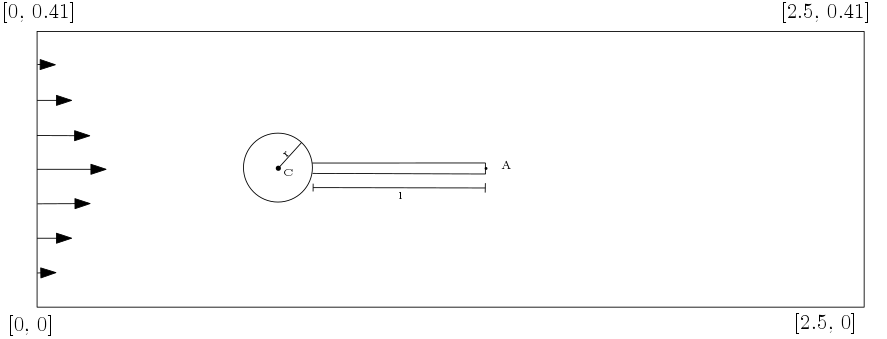
\includegraphics[scale=0.2]{./Fig/turekflag.png}
      \caption{Computational domain of the validation benchmark.}
      \label{fig:tflag}
\end{figure}
The benchmark is divided into three problems, each further divided into three different sub-problems with increasing complexity. In the first problem, the fluid solver is tested for different inlet flow profiles. The second problem considers the structure solver, evaluating the bending of the elastic flag. And the final problem concerns validation of a full fluid-structure interaction problem with the fluid and the elastic flag.  Several quantities for comparison are presented in \cite{Hron2006} for validation purposes:
\begin{itemize}
\item The position (x,y) of point A(t) as the elastic flag undergoes deformation.
\item Drag and lift forces exerted on of the whole interior geometry in contact with the fluid, consisting of the rigid circle and the elastic beam.
\begin{align*}
(F_D, F_L) = \int_{\Gamma} \mathbf{\sigma} \cdot \mathbf{n} dS
\end{align*}
\end{itemize}
\newpage
All problems pose both steady state and periodic solutions. For the steady state solutions, the quantity of interest will be calculated based on a transient simulation, that has converged towards a steady state solution. For the periodic solutions, the amplitude and mean values for the time dependent quantity are calculated from the last period.
\begin{align}
\text{mean} = \frac{1}{2} \text{max + min} \\
\text{amplitude} = \frac{1}{2} \text{max - min}
\label{icond}
\end{align}
 In \cite{Hron2006}, all steady state solutions seems to be calculated by solving a steady state equation since time-step are only reported for the periodic solutions. In this thesis, all problems in \cite{Hron2006} are calculated using time integration. The main reason for solving the problem transiently rather than steady state, is that numerical errors associated with initial transients are negligible with a sufficiently low time step size, without laborious changes to the numerical implementation. In the following section, an overview of each problem together with numerical results will be presented. A discussion of the results are given at the end of each simulation problem. For each table, the relative error of the finest spatial and temporal refinement compared to the reference solution is reported in \cite{Hron2006}.
 \newpage
\subsection{Validation of fluid solver}
The validation test of the fluid solver addresses transient flow for a low Reynolds-number regime. We can take to different approaches to this problem \cite{Hron2006}. The first one considers the setup as a fluid-structure interaction problem, setting the material properties to mimic a stiff rod. In the second approach, the flag is excluded from the computational domain. Thus, any influence from the structure is eliminated. In this thesis, I choose to use second approach.  \\
\textit{Let $\mathbf{v}_f$, ${p}_f$ be the fluid velocity and pressure, and let  $\sigma_f$ be the Cauchy stress tensor, and $\mathbf{f}_f$ denote any sourceterm,  Find $\mathbf{v}_f$, ${p}_f$ such that }:
\begin{align*}
 \big( \pder{\mathbf{v}_f}{t}, \ \bm{\psi}^u \big)_{\hat{\Omega}_f} +
\feme{(\mathbf{v}_f \cdot \nabla) \mathbf{v}_f}{\bm{\psi}^u}
- \feme{\hat{\sigma}}{\nabla\bm{\psi}^u} -
\feme{\rho_f  \mathbf{f}_f}{{\bm{\psi}^u}} = 0 \\
\feme{\nabla \cdot \mathbf{v}_f)}{\bm{\psi}^p} = 0 
\end{align*} 
\begin{table}[h!]
\centering
\begin{tabular}{ |p{3cm}||p{2cm}|p{2cm}|p{2cm}|  }
\hline
 parameter              & CFD-1 & CFD-2 & CFD-3 \\
 \hline
$\rho^f [10^{3}\frac{kg}{m^3}]$ & 1    & 1    & 1    \\
$\nu^f  [10^{-3}\frac{m^2}{s}]$  & 1    & 1    & 1    \\
U                      & 0.2  & 1    & 2    \\
Re                     & 20   & 100  & 200 \\
\hline
\end{tabular}
\caption{Parameters for the fluid validation set-up. Note that only the inlet velocity is changing.}
\label{sec:cfdparam}
\end{table}
The validation of the fluid solver is divided into three sub-problems; CFD-1, CFD-2, and CFD-3, each with different fluid parameters shown in Table ~\ref{sec:cfdparam}. While CFD-1 and CFD-2 are steady state solutions, it is expected that the CFD-3 results is temporally varying with a von Karman street behind the flag. A parabolic velocity profile on the form,
\begin{align*}
v_f(0, y) = 1.5 U\frac{(H -y)y}{(\frac{H}{2})^2}
\end{align*}
is set on the left channel inflow. H is the height of the channel, while the parameter U is set differently to each problem to induce different inlet flow profiles. At the channel outflow, the pressure is set to $p = 0$. No-slip boundary conditions for the fluid are enforced on the channel walls, and on the inner geometry consisting of the circle and the elastic flag. The validation of the fluid solver is based on the evaluation of drag and lift forces on the inner geometry, compared against a reference solution. A spatial and temporal convergence study is conducted on all sub-problems. 
\newpage
\subsubsection*{Results}
Table ~\ref{table:cfd1}, ~\ref{table:cfd2}, and ~\ref{table:cfd32} below shows the numerical solution of each sub-problem, CFD-1, CFD-2, and CFD-3. Each sub-problem is evaluated on four different mesh with increasing resolution. For the numerical solution of CFD-3 in Table 4.4, additional temporal and spatial refinement studies are conducted. Figure 4.1 shows the evaluation of lift and drag for the finest spatial and temporal resolution, while Figure 4.3 shows a visual representation of the fluid flow through the channel. The numerical solutions of CFD-1 in Figure 4.2 shows convergence against the reference solution. Choosing P2-P1 elements together with a fully implicit scheme $\theta = 1$, a relative error of $0.006 \%$ for lift, and $0\%$ for drag is attained. For the numerical solution of CFD-2 presented in Figure 4.3, the same observations apply. The second order Crank-Nicolson scheme  $\theta = 0.5$ was investigated for CFD-1 and CFD-2, however only improving the results of order $10^{-6}$ for both lift and drag. For the periodic problem CFD-3, the choice of  P2-P1 elements with a fully implicit time-stepping scheme proved insufficient for capturing the expected periodic solution. Using Crank-Nicolson time-stepping scheme $\theta = 0.5$, the periodic solution was attained. 
\begin{table}[h!]
\centering
\begin{tabular}{ |p{1cm}||p{2.7cm}|p{3.3cm}|p{3.3cm}|}
\hline
  \multicolumn{4}{|c|}{$\Delta t = 0.1 \hspace{2mm} \theta = 1.0$} \\
\hline
nel & ndof & Drag  & Lift \\
\hline
 1438    & 6881   & 13.60 & 1.089  \\
 2899    & 13648  & 14.05 & 1.126 \\
 7501    & 34657  & 14.17   & 1.109 \\
 19365   & 88520  & 14.20 & 1.119 \\
  \hline
  \multicolumn{2}{|c|}{Reference}  & 14.29   & 1.119\\
   \hline
    \multicolumn{2}{|c|}{Error}  & 0.006 \%   & 0.00 \%\\
   \hline
\end{tabular}
\caption{CFD-1 results, lift and drag evaluated at the inner geometry surface for increasing spatial refinement. The error is computed as the relative error from the highest mesh resolution against the reference solution.}
\label{table:cfd1}
\end{table}
\begin{table}[h!]
\centering
\label{CFD-2 Results}
\begin{tabular}{ |p{1cm}||p{2.7cm}|p{3.3cm}|p{3.3cm}|}
 \hline
  \multicolumn{4}{|c|}{$\Delta t = 0.01 \hspace{2mm} \theta = 1.0$} \\
   \hline
nel & ndof & Drag  & Lift \\
\hline
 1438    & 6881 (P2-P1)  & 126.0 &  8.62 \\
 2899    & 13648  (P2-P1)& 131.8 & 10.89  \\
 7501    & 34657 (P2-P1) & 135.1 & 10.48  \\
 19365   & 88520(P2-P1)  & 135.7 & 10.55  \\
 \hline
  \multicolumn{2}{|c|}{Reference}  & 136.7   & 10.53\\
   \hline
    \multicolumn{2}{|c|}{Error}  & 0.007 \%   & 0.001 \%\\
   \hline
\end{tabular}
\caption{CFD-2 results, lift and drag evaluated at the inner geometry surface for increasing spatial refinement. The error is computed as the relative error from the highest mesh resolution against the reference solution.}
\label{table:cfd2}
\end{table}
\begin{figure}[h!]
  \centering
    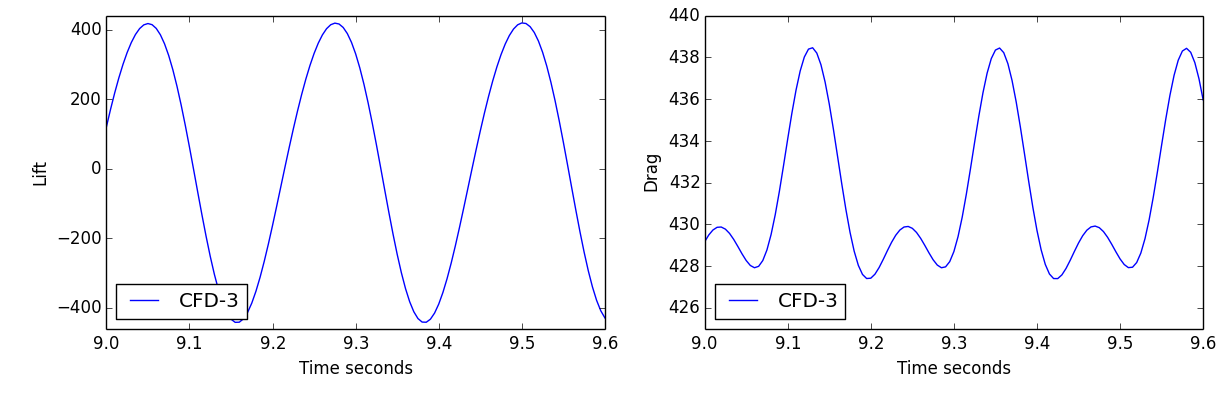
\includegraphics[scale=0.5]{./Fig/cfd3_liftdrag.png}
      \caption{CFD-3, lift and drag forces at time t = [9, 9.6].}
\end{figure}
\begin{figure}[h!]
  \centering
    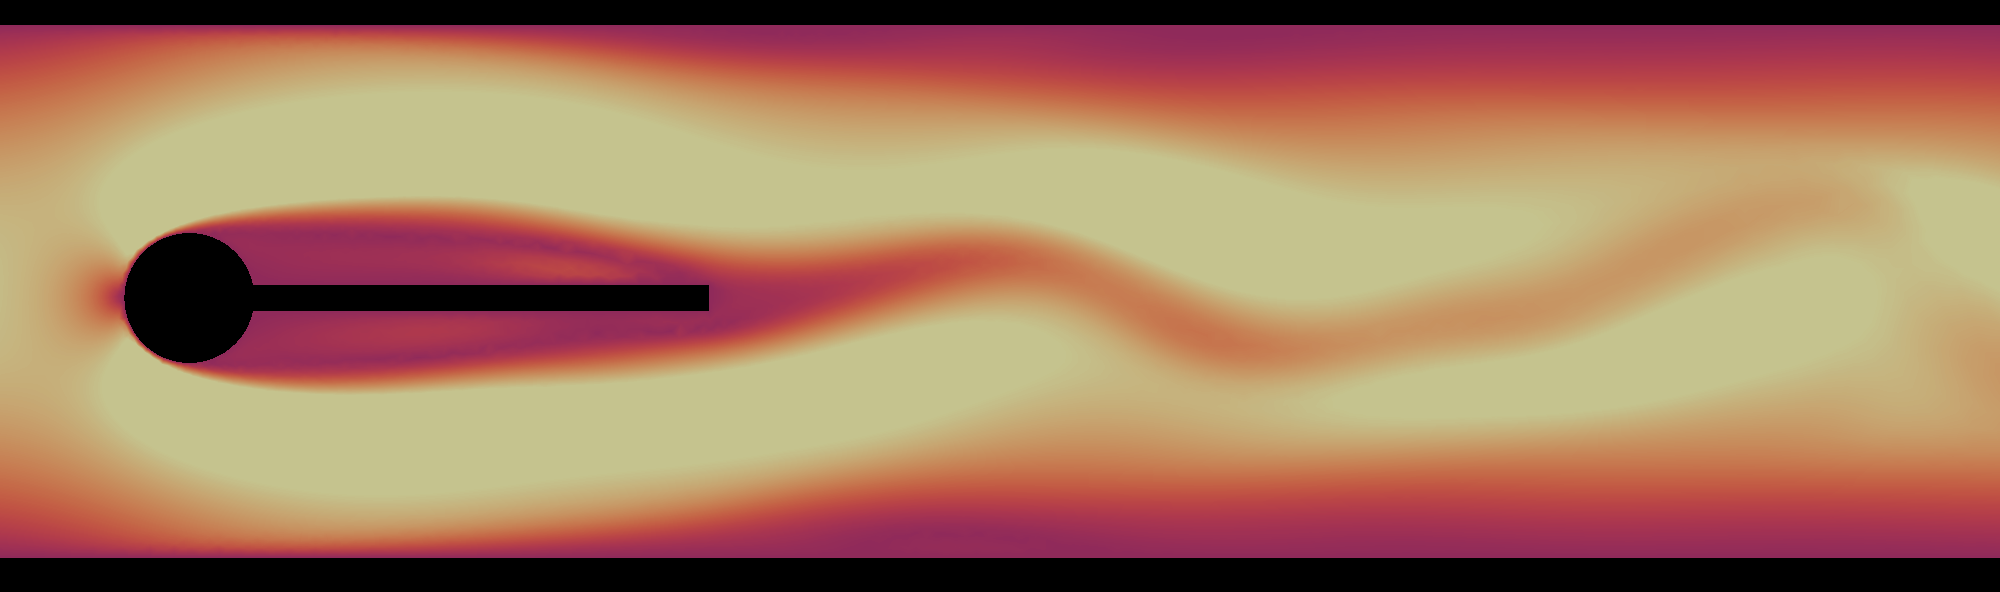
\includegraphics[scale=0.2]{./Fig/cfd3.png}
      \caption{CFD-3, flow visualization of velocity time t = 9s.}
\end{figure}
\newpage
\begin{table}[h!]
\centering
\label{CFD-3 Results}
\begin{tabular}{ |p{1cm}||p{2.9cm}|p{3.3cm}|p{3.3cm}|}
 \hline
  \multicolumn{4}{|c|}{$\Delta t = 0.01 \hspace{2mm} \theta = 0.5$} \\
   \hline
nel & ndof & Drag  & Lift \\
\hline
 1438    & 6881  (P2-P1)   & 417.23       $\pm$   0.0217 & -249.21   $\pm$  0.32  \\
   & 16474 (P3-P2)   & 414.86      $\pm$  5.6282 & -7.458      $\pm$  444.07  \\
 \hline
 2899    & 13648  (P2-P1) & 408.50  $\pm$   4.3029 & -19.731  $\pm$   373.45 \\  
     &  32853 (P3-P2)  & 432.86      $\pm$  5.5025 & -9.686      $\pm$  431.28  \\
  \hline
  7501    & 34657 (P2-P1) & 431.57  $\pm$   5.2627 & -12.497  $\pm$   429.76 \\    
    &  83955 (P3-P2)  & 438.20      $\pm$  5.5994 & -11.595      $\pm$  438.00 \\
    \hline
    19365   & 88520 (P2-P1) & 435.43  $\pm$   5.4133 & -11.545  $\pm$   438.89 \\
   &   215219 (P3-P2) & 438.80      $\pm$  5.6290 & -11.158      $\pm$  439.23 \\
\hline
 \multicolumn{2}{|c|}{Reference}  & 439.95 $\pm$ 5.6183 & -11.893 $\pm$ 437.81\\
 \hline
  \multicolumn{2}{|c|}{Error}  & 0.002 \% $\pm$ 0.001 \% & 0.061 \% $\pm$ 0.003\% \\
  \hline
  \end{tabular}
\end{table}
\begin{table}[h!]
\centering
\label{CFD-32 Results}
 \begin{tabular}{ |p{1cm}||p{2.9cm}|p{3.3cm}|p{3.3cm}|}
  \hline
  \multicolumn{4}{|c|}{$\Delta t = 0.005 \hspace{2mm} \theta = 0.5$} \\
   \hline
nel & ndof & Drag  & Lift \\
\hline
 1438    & 6881  (P2-P1)   &  417.24  $\pm$  0.0084 & -249.386   $\pm$ 0.1345  \\
 1438    & 16474 (P3-P2)   & 414.90     $\pm$  5.7319 & -8.467 $\pm$  443.45  \\
\hline
 1438    &13648  (P2-P1)   & 408.27   $\pm$ 4.0192 & -18.981   $\pm$ 363.84 \\
 2899    &  32853 (P3-P2)   & 432.90      $\pm$  5.5333 & -11.382      $\pm$  430.60 \\
 \hline
 1438    & 34657  (P2-P1)   & 431.59 $\pm$5.2979 & -13.644   $\pm$ 429.68 \\
 7501    & 83955 (P3-P2)  & 438.23      $\pm$  5.6393 & -12.917 $\pm$  437.78 \\
 \hline
 1438    & 88520  (P2-P1)   & 435.46  $\pm$ 5.4579 & -13.190   $\pm$ 438.05 \\
 19365   & 215219 (P3-P2)  & 438.84    $\pm$  5.6576 & -12.786      $\pm$  438.36 \\
\hline
 \multicolumn{2}{|c|}{Reference}  & 439.95 $\pm$ 5.6183 & -11.893 $\pm$ 437.81\\
 \hline
  \multicolumn{2}{|c|}{Error}  & 0.002 \% $\pm$ 0.006 \% & 0.075 \% $\pm$ 0.001\% \\
  \hline
\end{tabular}
\caption{CFD-3 results, lift and drag evaluated at the inner geometry surface. A spatial refinement study is conducted for increasing mesh resolution and two different finite element pairs. The relative error is computed from the solution of the highest mesh resolution, against the reference solution.}
\label{table:cfd32}
\end{table}
\subsubsection*{Discussion}
Since the choice of finite-element pair is not reported in the original work, both P3-P2 and P2-P1 element pairs for fluid and pressure respectively was compared in combination with spatial mesh refinement. From Table 4.3, a relative error $ < 0.08\%$ of the mean and amplitude for lift and drag is attained. The choice P3-P2 element pair is eminent to achieve reasonable results for the first and second mesh regardless of time step.  However, the third and fourth mesh resolution shows close resemblance with the reference solution, independent of finite-element pair. On basis of the presented results, the fluid solver is validated in accordance with the proposed benchmark. 
\subsection{Validation of solid solver}
The validation of the solid solver is conducted on a rectangular domain, representing the elastic structure in Figure ~\ref{fig:tflag}.  The structure is fixed to a fictional wall on the left side of the domain, pulled by a gravitational force $\mathbf{g} = (0, g)$. The validation of the solid solver is based on comparison of the deflection of point $A(t) = [A_x(t), A_y(t)]$,  conducted on three refined mesh, where the number of finite elements are chosen in close resemblance with the original work in \cite{Hron2006}. A simple investigation of different finite-element pairs, suggest that P3-P3 elements where used for making the reference solution. In this study, lower order finite-element pair was included, comparing shorter simulation time with solution accuracy. While computational time is not a major concern for the solid solver, the study is important for potentially reducing the computational time for the final validation problem.
\begin{table}[h!]
\centering.
\label{my-label}
\begin{tabular}{ |p{3cm}||p{2cm}|p{2cm}|p{2cm}|  }
 \hline
 parameter              & CSM 1 & CSM 2 & CSM 3 \\
 \hline
$\rho^s [10^{3}\frac{kg}{m^3}]$ & 1    & 1    & 1    \\
$\nu^s $  & 0.4    & 0.4    & 0.4    \\
$\mu^s  [10^{6}]$  & 0.5    & 2.0    & 0.5    \\
$g  \frac{m}{s^2}]$  & 2.0    & 2.0    & 2.0    \\
\hline
\end{tabular}
\caption{Parameters for the solid validation set-up.}
\end{table}
\subsubsection*{Results}
The numerical results for CSM-1, CSM-2, and CSM-3 are presented in table  ~\ref{table:csm1}, ~\ref{table:csm2}, ~\ref{table:csm31}, and ~\ref{table:csm32}. For the steady state sub-problems CSM-1 and CSM-2, a spatial convergence study is conducted through mesh refinement with three different finite-element pairs. For the periodic CSM-3 problem, an additional temporal study was conducted for two different time steps. In Figure ~\ref{fig:bender}, a visualization of CSM-3 is provided for three different time steps. Finally, Figure ~\ref{fig:csm3c} shows the displacement vector components, comparing all finite-element pairs for the finest mesh resolution. \\
 For CSM-1, the relative error of deformation found in Table 4.6, is $1.41 \%$ and $0.8\%$ for the x and y coordinate respectively. In Table 4.7, a relative error of   $1.49 \%$ and $0.88\%$ for the x,y components can be found for CSM-2, proving both steady state problems coincide with the reference solution. In Table 4.8, the numerical solutions CSM-3 for time steps $\Delta t = 0.01$ and $\Delta t = 0.005$, are in close resemblance with the reference solution. The study of lower-order elements proved successful for all problems, justifying accurate results can be achieved using P2-P2 elements for deformation and velocity, even for coarse mesh resolution. 
 
\begin{table}[h!]
\centering
\begin{tabular}{ |p{1cm}||p{2.7cm}|p{3.3cm}|p{3.3cm}|}
\hline
  \multicolumn{4}{|c|}{$\Delta t = 0.1 \hspace{2mm} \theta = 1.0$} \\
\hline
nel & ndof & ux of A [x $10^{-3}$]  &uy of A [x $10^{-3}$] \\
\hline
 319     & 832 P1-P1  & -5.278 &  -56.6 \\
     & 2936 P2-P2 & -7.056 &  -65.4 \\
      & 6316 P3-P3 &  -7.064 &   -65.5  \\
 \hline
  1365    & 3140 P1-P1  & -6.385 &  -62.2 \\
     & 11736 P2-P2 & -7.075 &  -65.5 \\
     & 25792 P3-P3 & -7.083 &  -65.5 \\
 \hline
  5143    & 11084 P1-P1 & -6.905 &  -64.7  \\
     & 42736 P2-P2 & -7.083 &  -65.4\\
     & 94960 P3-P3 & -7.085 &  -65.5  \\
  \hline
  \multicolumn{2}{|c|}{Reference}  &-7.187    & -66.1 \\
   \hline
    \multicolumn{2}{|c|}{Error}  & 1.41 \%   & 0.8 \%\\
   \hline
\end{tabular}
\caption{CSM-1, deformation components of A(t) for $\Delta t = 0.1$ and increasing spatial refinement. The error is computed as the relative error from the highest mesh resolution against the reference solution.}
\label{table:csm1}
\end{table}
\begin{table}[h!]
\centering
\begin{tabular}{ |p{1cm}||p{2.7cm}|p{3.3cm}|p{3.3cm}|}
\hline
  \multicolumn{4}{|c|}{$\Delta t = 0.05 \hspace{2mm} \theta = 1.0$} \\
\hline
nel & ndof & ux of A [x $10^{-3}$]  &uy of A [x $10^{-3}$] \\
\hline
 319     & 832 P1-P1  & -0.3401 &  -14.43  \\ 
     & 2936 P2-P2 &  -0.460  &  -16.78  \\ 
      & 6316 P3-P3 & -0.461 &  -16.79  \\
        \hline
  1365    & 3140 P1-P1  &  -0.414 &  -15.93\\
     & 11736 P2-P2 &  -0.461 &  -16.81 \\
     & 25792 P3-P3 & -0.461  &  -16.82 \\
        \hline
   5143    & 11084 P1-P1 & -0.449 &  -16.60  \\
     & 42736 P2-P2 &-0.461 &  -16.82 \\
     & 94960 P3-P3 & -0.462 &  -16.82 \\
  \hline
  \multicolumn{2}{|c|}{Reference}  & -0.469      & -16.97  \\
   \hline
    \multicolumn{2}{|c|}{Error}  & 1.49\%   & 0.88 \%\\
   \hline
\end{tabular}
\caption{CSM-2, deformation components of A(t) for $\Delta t = 0.05$ and increasing spatial refinement. The error is computed as the relative error from the highest mesh resolution against the reference solution.}
\label{table:csm2}
\end{table}
\newpage
\begin{table}[h!]
\centering
\begin{tabular}{ |p{1cm}||p{2.7cm}|p{3.3cm}|p{3.3cm}|}
\hline
  \multicolumn{4}{|c|}{$\Delta t = 0.01 \hspace{2mm} \theta = 0.5$} \\
\hline
nel & ndof & ux of A [x $10^{-3}$]  &uy of A [x $10^{-3}$] \\
\hline
    319     & 832 P1-P1 & -10.835       $\pm$   10.836 & -55.197    $\pm$  56.845 \\
     & 2936 P2-P2 & -14.390       $\pm$   14.392 & -63.303      $\pm$   65.149 \\
      & 6316 P3-P3& -14.432      $\pm$   14.435 & -63.397   $\pm$   65.263 \\
    \hline
    1365    & 3140 P1-P1  & -13.053     $\pm$   13.054 & -60.367      $\pm$ 62.241 \\
     & 11736 P2-P2  & -14.428       $\pm$  14.432 & -63.388   $\pm$   65.256 \\
     & 25792 P3-P3  & -14.444      $\pm$   14.446 & -63.432    $\pm$   65.287 \\
     \hline
     5143    & 11084 P1-P1 & -14.082       $\pm$  14.084 & -62.656   $\pm$   64.495 \\
     & 42736 P2-P2 & -14.444     $\pm$  14.447 & -63.435   $\pm$   65.288 \\
     & 94960 P3-P3& -14.449      $\pm$  14.452 & -63.449    $\pm$   65.296 \\
 \hline
  \multicolumn{2}{|c|}{Reference}  &-14.305 +- -14.305        & -63.607 +- 65.160    \\
   \hline
    \multicolumn{2}{|c|}{Error}  & 1\% $\pm$ 1\%   & 0.24\% $\pm$ 0.24\%\\
   \hline
\end{tabular}
\caption{CSM-3, deformation components of A(t) for $\Delta t = 0.01$, with increasing temporal refinement. The error is computed as the relative error from the highest mesh resolution.}
\label{table:csm31}
\end{table}
\begin{table}[h!]
\centering
\begin{tabular}{ |p{1cm}||p{2.7cm}|p{3.3cm}|p{3.3cm}|}
\hline
  \multicolumn{4}{|c|}{$\Delta t = 0.005 \hspace{2mm} \theta = 0.5$} \\
\hline
nel & ndof & ux of A [x $10^{-3}$]  &uy of A [x $10^{-3}$] \\
\hline
    319     & 832 P1-P1 & -10.846     $\pm$ 10.848 & -56.049    $\pm$   56.053 \\
     & 2936 P2-P2  & -14.390     $\pm$  14.391 & -63.738       $\pm$  64.703 \\
      & 6316 P3-P3 & -14.429     $\pm$  14.430 & -63.833       $\pm$   64.810 \\
 \hline 
    1365    & 3140 P1-P1 & -13.057     $\pm$   13.057 & -60.813       $\pm$  61.826 \\
     & 11736 P2-P2& -14.426     $\pm$   14.427 & -63.827       $\pm$   64.801 \\
     & 25792 P3-P3 & -14.440     $\pm$ 14.441 & -63.854      $\pm$  64.845 \\
 \hline
      5143    & 11084 P1-P1 & -14.091      $\pm$  14.091 & -63.195    $\pm$  63.981 \\
     & 42736 P2-P2 & -14.441      $\pm$   14.441 & -63.856    $\pm$  64.847 \\
     & 94960 P3-P3 & -14.446     $\pm$ 14.446 & -63.865      $\pm$   64.860 \\
 \hline
  \multicolumn{2}{|c|}{Reference}  &-14.305 +- -14.305        & -63.607 +- 65.160    \\
   \hline
    \multicolumn{2}{|c|}{Error}  & 1\% $\pm$ 1\% &  0.4\% $\pm$ 0.4\%  \\
   \hline
\end{tabular}
\caption{CSM-3, deformation components of A(t) for $\Delta t = 0.005$, with increasing temporal refinement. The error is computed as the relative error from the highest mesh resolution.}
\label{table:csm32}
\end{table}
\newpage
\begin{figure}
    \centering
    \begin{subfigure}[b]{0.3\textwidth}
        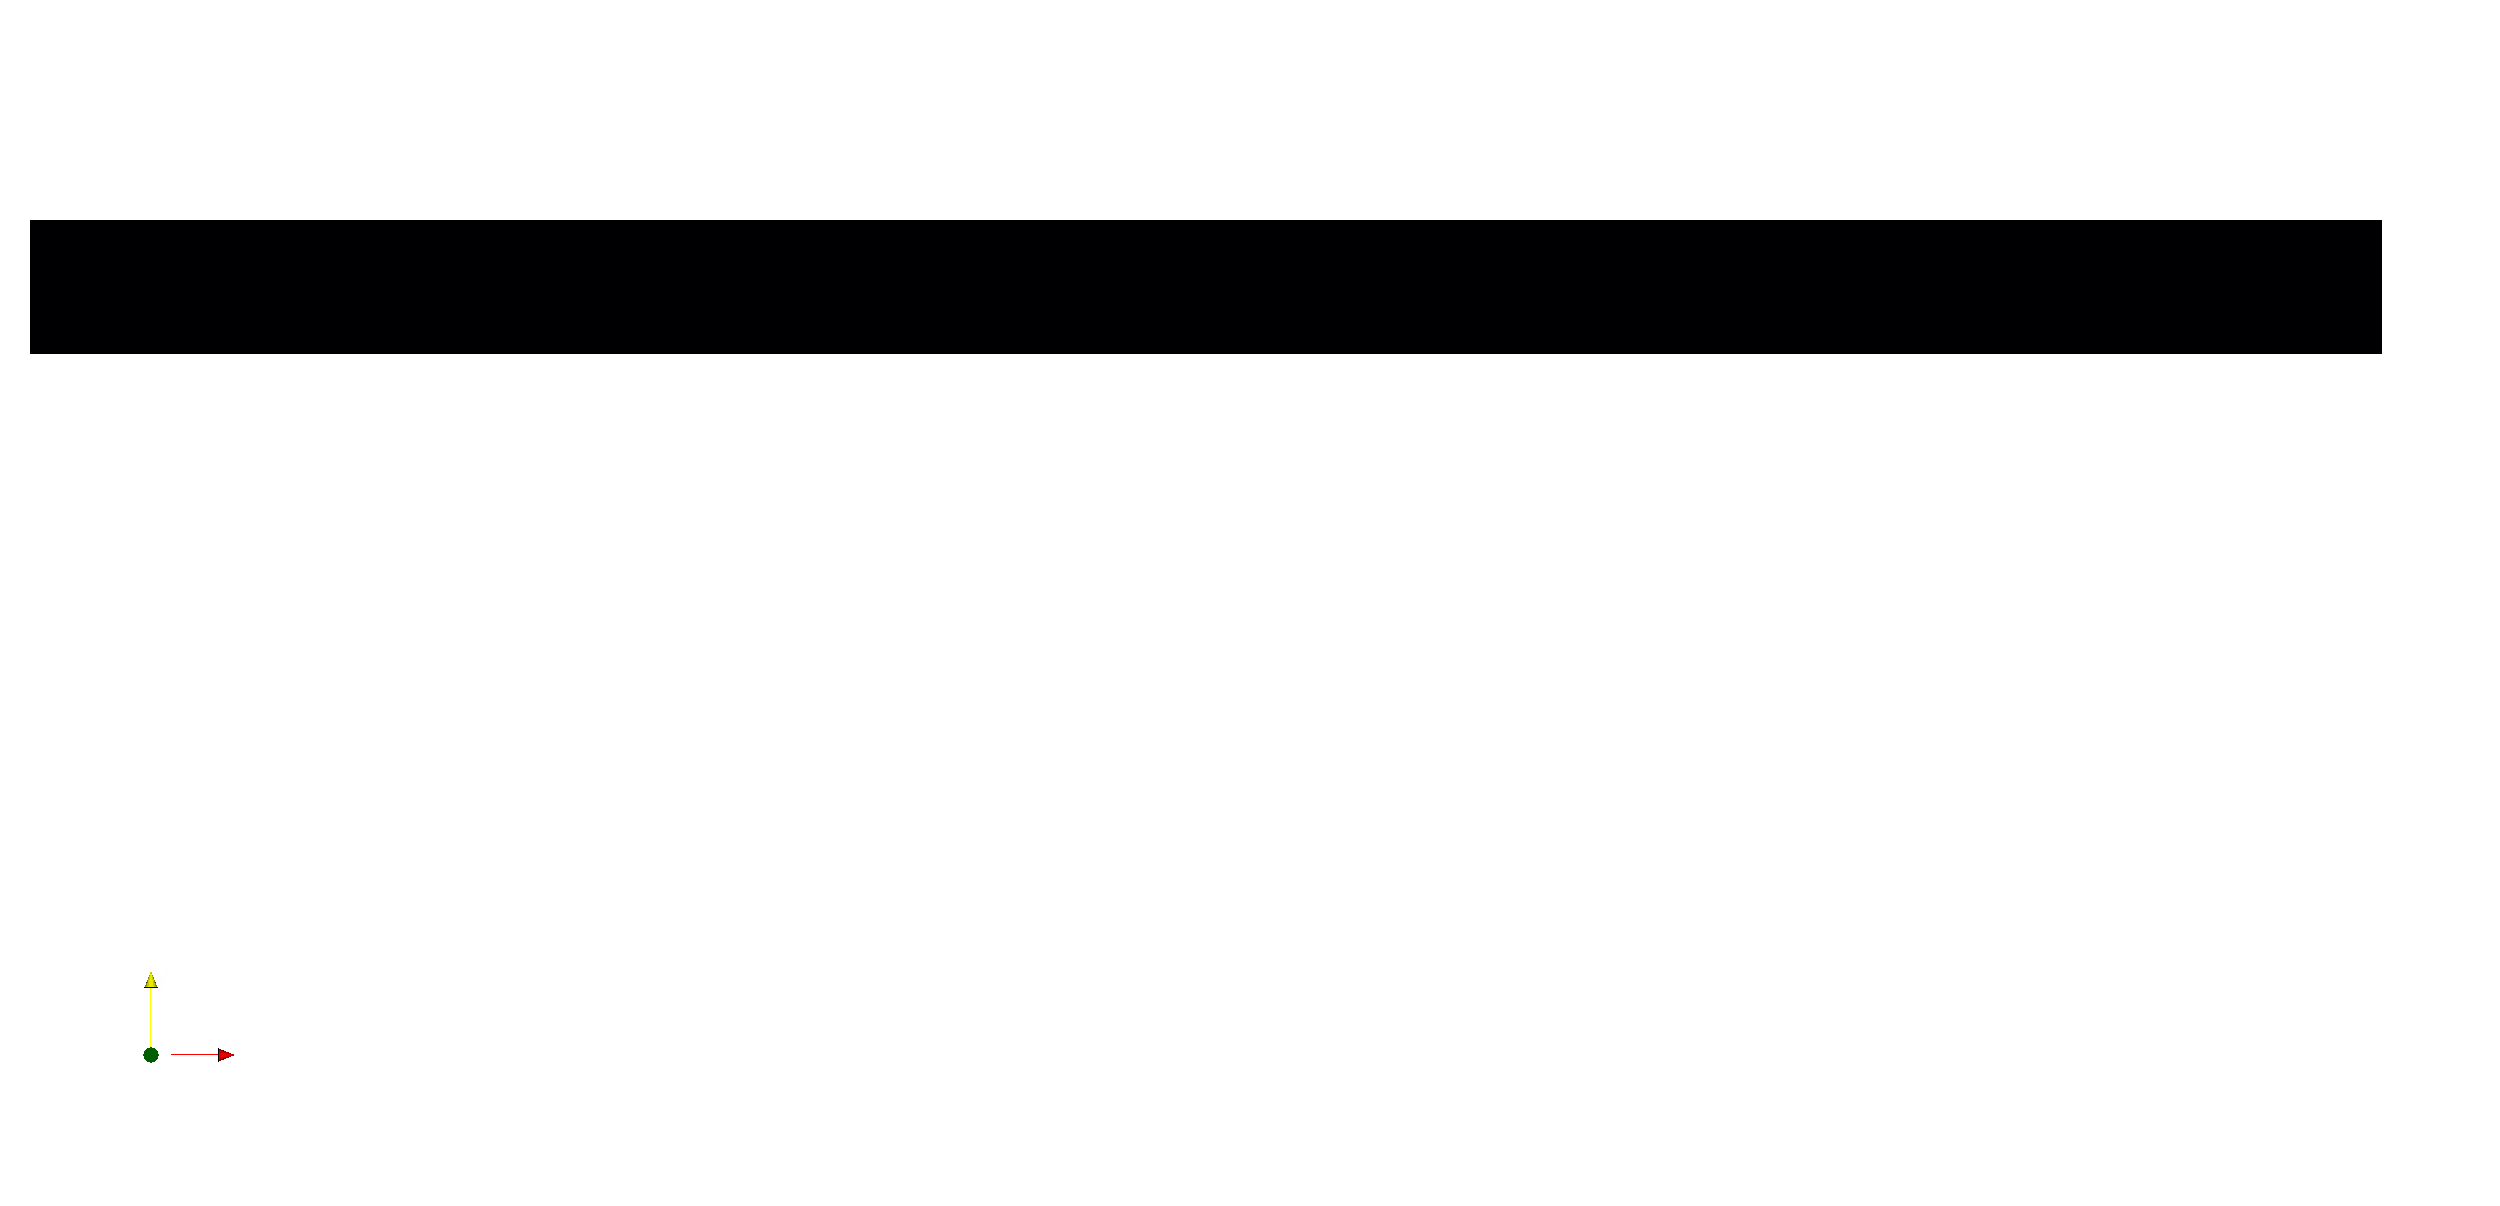
\includegraphics[width=\textwidth]{./Fig/csm3_1.png}
       \caption{$t = 0$}
        \label{fig:gull}
    \end{subfigure}
    ~ %add desired spacing between images, e. g. ~, \quad, \qquad, \hfill etc. 
      %(or a blank line to force the subfigure onto a new line)
    \begin{subfigure}[b]{0.3\textwidth}
        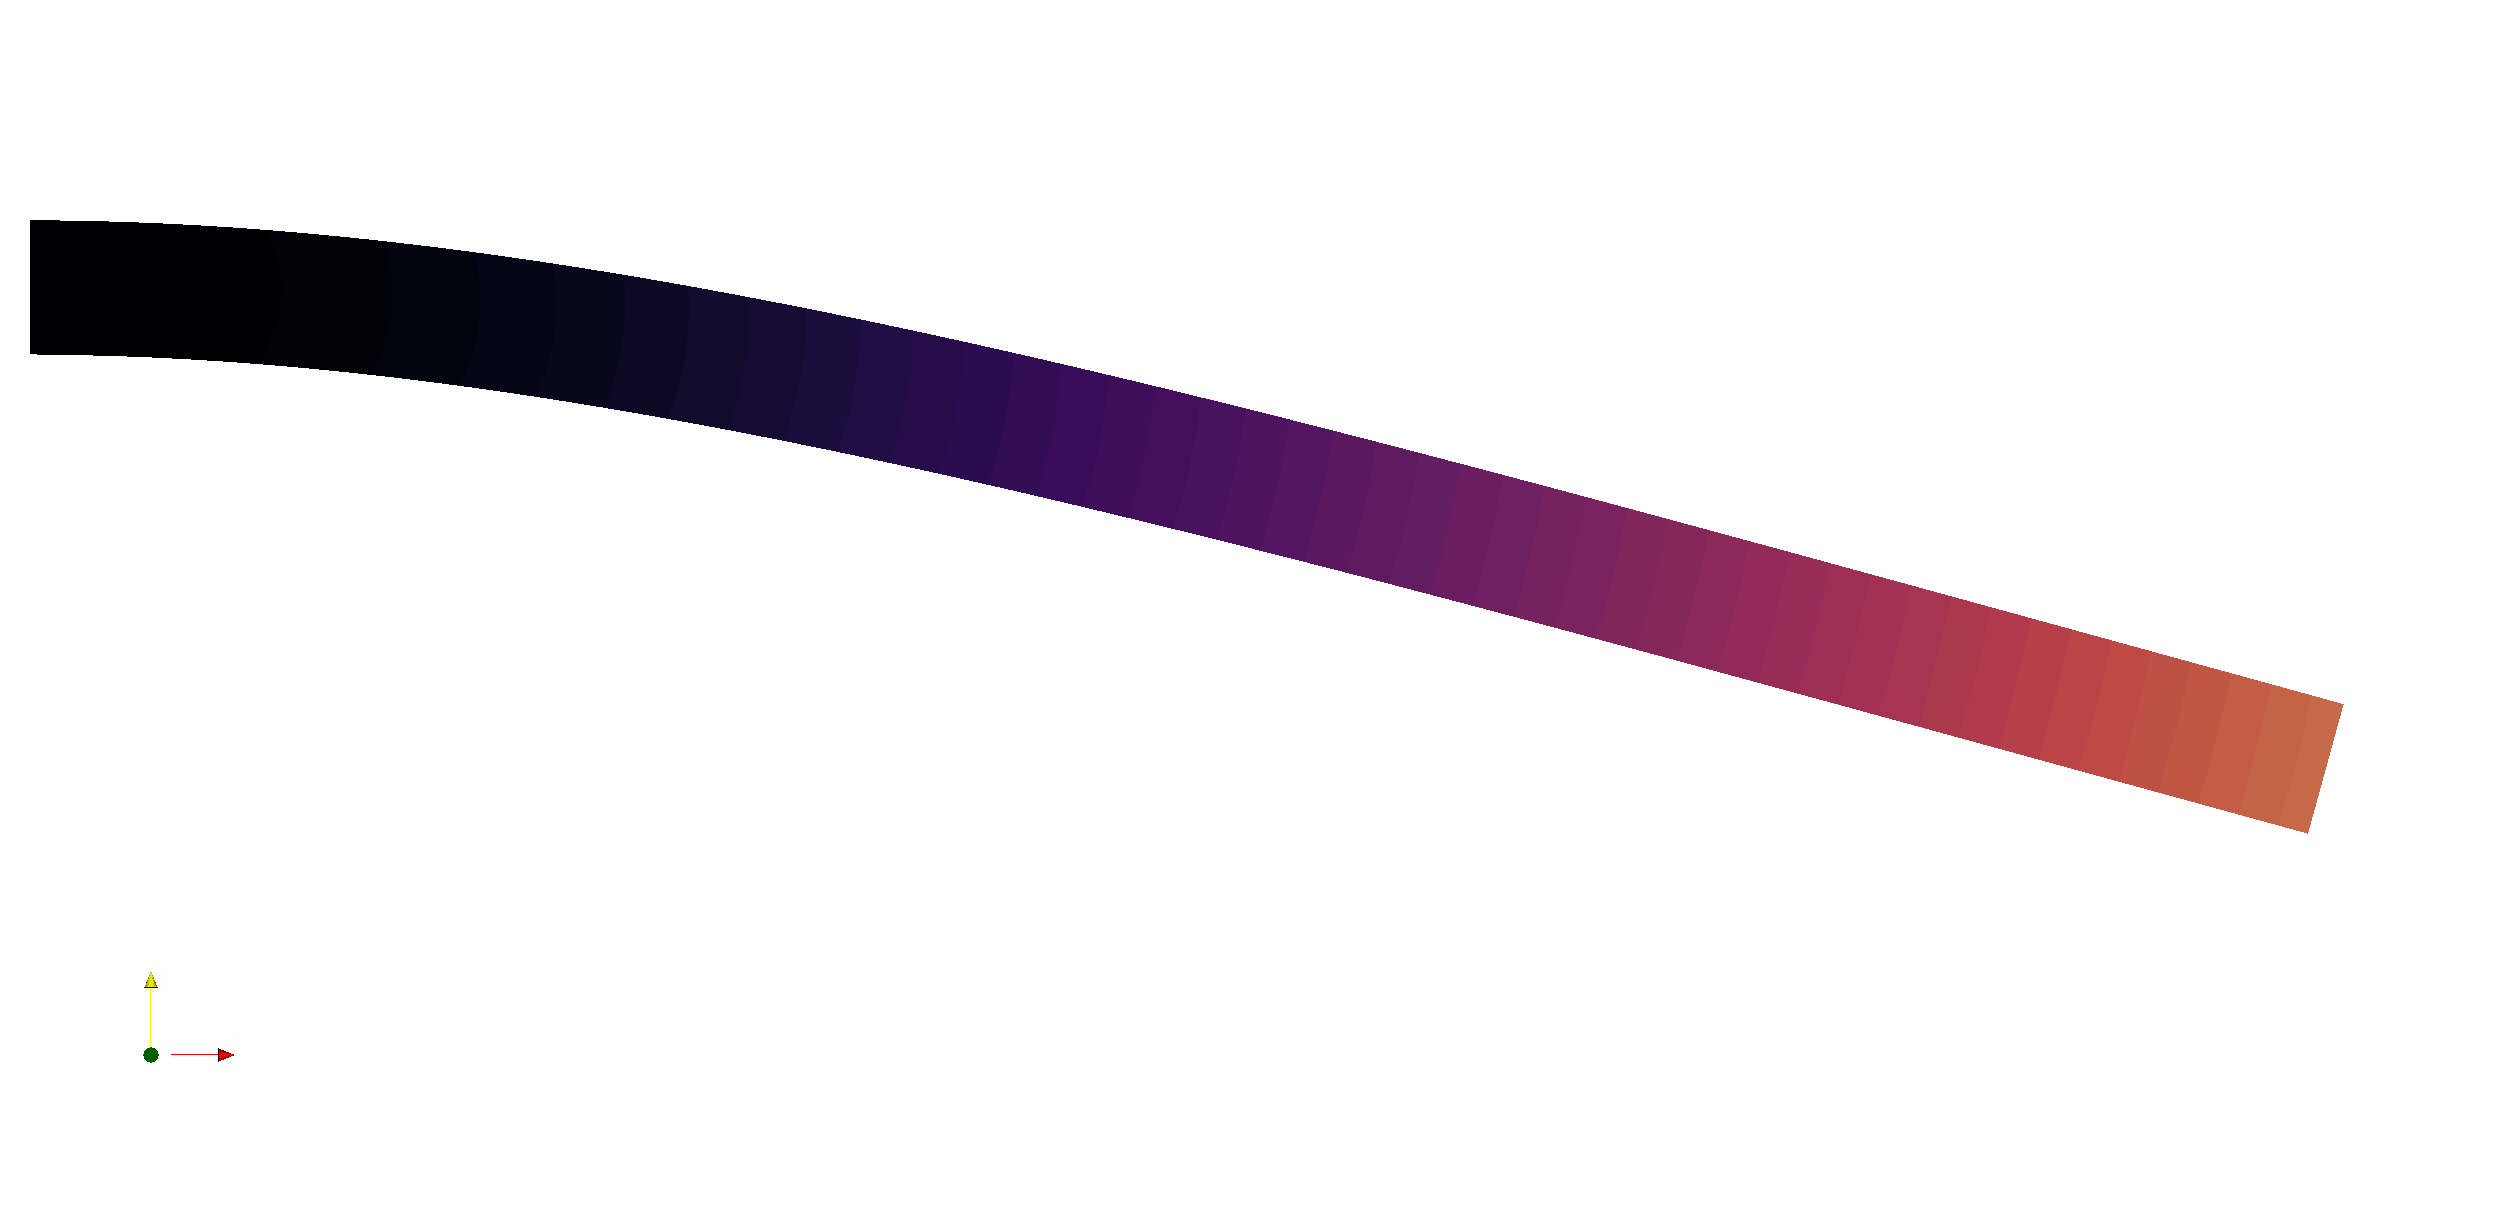
\includegraphics[width=\textwidth]{./Fig/csm3_2.png}
               \caption{$t = 0.22$}
        \label{fig:tiger}
    \end{subfigure}
    ~ %add desired spacing between images, e. g. ~, \quad, \qquad, \hfill etc. 
    %(or a blank line to force the subfigure onto a new line)
    \begin{subfigure}[b]{0.3\textwidth}
        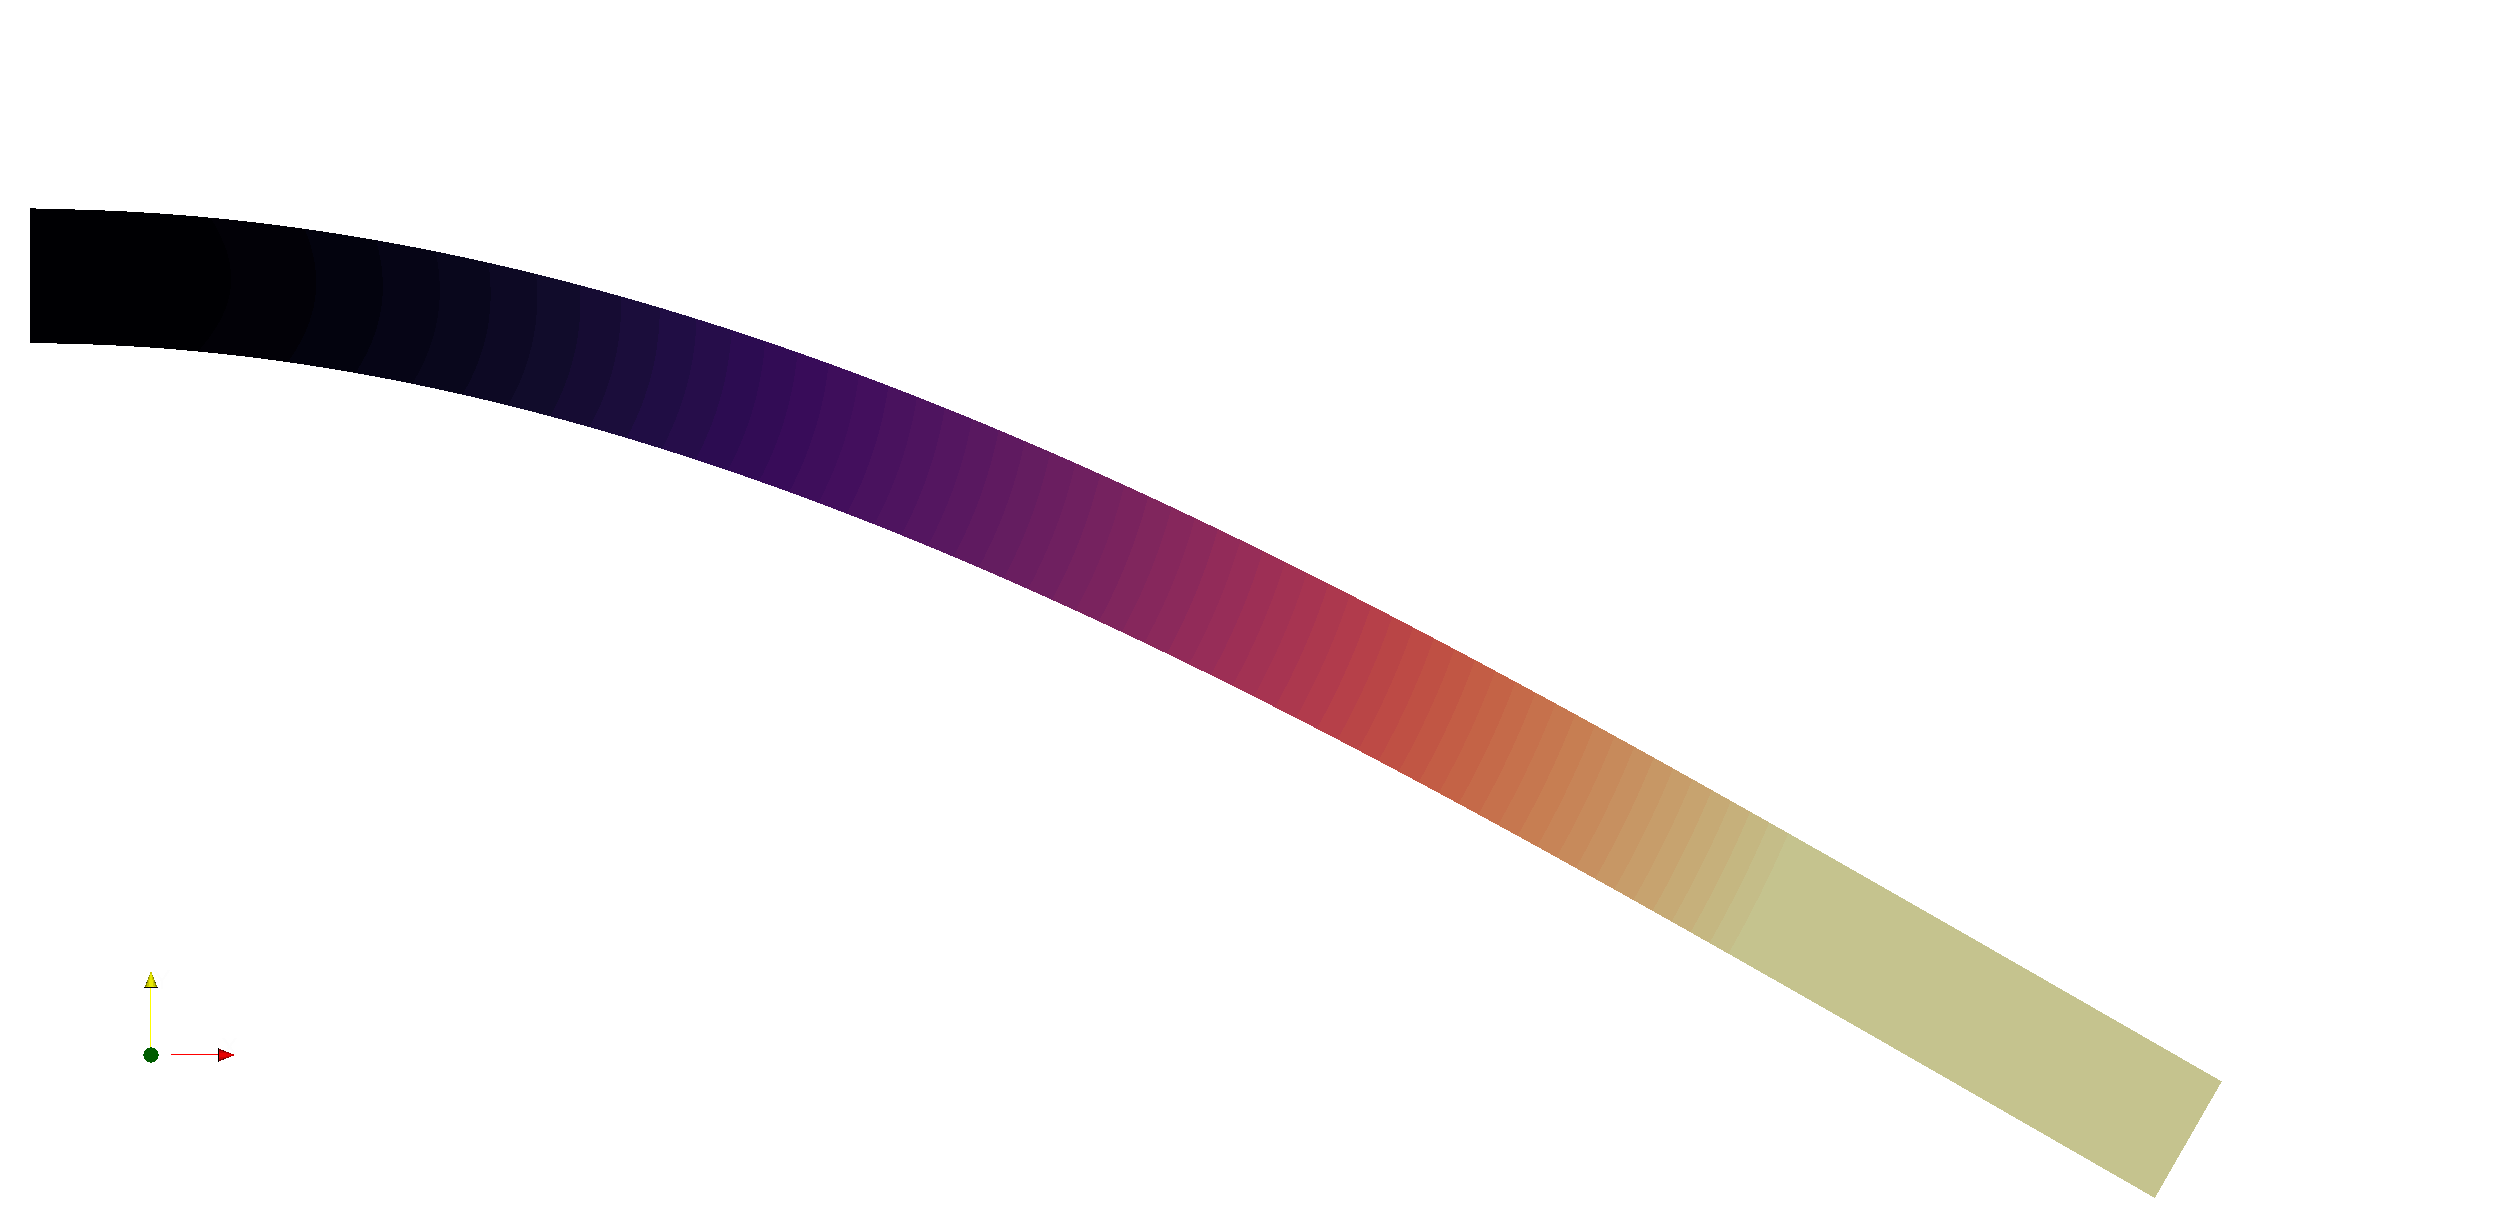
\includegraphics[width=\textwidth]{./Fig/csm3_3.png}
        \caption{$t = 0.45$}
        \label{fig:mouse}
    \end{subfigure}
    \caption{CSM-3, visualization of deformation of the elastic flag for three time steps: (a) initial configuration, (b) half way extension, (c) full extension }
 \label{fig:bender}
\end{figure}
\begin{figure}[h!]
  \centering
    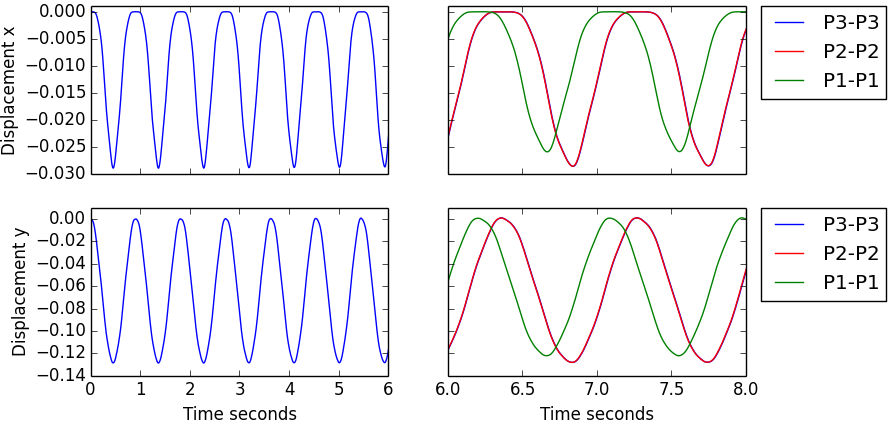
\includegraphics[scale=0.34]{./Fig/csm3compare.png}
      \caption{CSM-3 $\Delta t = 0.01$, deformation components of A(t) with finest mesh resolution, comparing all finite element pairs for time interval $t \in [0, 6]$  and $t \in [6, 8]$.}
       \label{fig:csm3c}
\end{figure}
\subsubsection*{Discussion}
 
 Comparing all finite-element pairs for CSM-3, visualized in figure 4.5, shows P2-P2 and P3-P3 elements hardly can be distinguished from each other. In accordance with previous mentioned results and observations, the solid solver is validated in accordance with the validation benchmark.
 
\subsection{Validation of fluid structure interaction solver}
\label{sec:fsi3}
The validation of the FSI solver consist of three sub-problems which will be referred to FSI-1, FSI-2 and FSI-3. The FSI-1 problem yields a steady state solution for the system, inducing small deformations to the elastic flag. The FSI-2 and FSI-3 problems results in a periodic solution, where the elastic flag oscillates behind the cylinder. All sub-problems inherit the conditions from the previous validation branches, with the exception of no gravitational force on the elastic flag. On the fluid-structure interface $\Gamma$, we enforce the kinematic and dynamic boundary condition
\begin{align}
\mathbf{v}_f = \mathbf{v}_s \\
\mathbf{\sigma}_f \cdot \mathbf{n} = \mathbf{\sigma}_s \cdot \mathbf{n}
\end{align}
Apart from the accuracy of the reported values, the main purpose of the validation of the solver is twofold. First, it is of great importance to ensure that the overall coupling of the fluid-structure interaction problem is executed correctly. Second, a good choice of mesh extrapolation model is essential to avoid divergence of the numerical solution, due to mesh entanglement.  Based on experience in section, 4.2.1-2, the finite element pair P2-P1 for the fluid solver, and P2-P2 for the solid solver proved successful. Therefore the finite-elements P2-P2-P1 for deformation, velocity, and pressure are chosen for the numerical experiments. Higher order elements will not be examined, mainly due to long computational time, even for optimized solver approaches.
\newpage
\begin{table}[h!]
\centering
\label{my-label}
\begin{tabular}{ |p{3cm}||p{2cm}|p{2cm}|p{2cm}|  }
 \hline
 \multicolumn{4}{|c|}{Solid parameters} \\
 \hline
 parameter              & FSI-1 & FSI-2 & FSI-3 \\
 \hline
 $\rho^s [10^{3} \frac{kg}{m^3}]$ & 1    & 10   & 1    \\
$\nu^s$ & 0.4  & 0.4  & 0.4  \\
$\mu^s  [10^{6}\frac{kg}{ms^2}]$  & 0.5  & 0.5  & 2.0  \\
 \hline
 \multicolumn{4}{|c|}{Fluid parameters} \\
 \hline
$\rho^f [10^{3}\frac{kg}{m^3}]$ & 1    & 1    & 1    \\
$\nu^f  [10^{-3}\frac{m^2}{s}]$  & 1    & 1    & 1    \\
U                      & 0.2  & 1    & 2    \\
parameter              & FSI-1 & FSI-2 & FSI-3 \\
Re                     & 20   & 100  & 200 \\
\hline
\end{tabular}
\caption{Fluid-structure interaction sub-problem parameters}
\end{table}
\subsubsection*{Results}
The numerical results for FSI-1, FSI-2, and FSI-3  are shown in Table 4.10-12. For all sub-problems, a spatial convergence study has been conducted on three different meshes with increasing resolution, with the relative error of the finest spatial and temporal resolution. For FSI-1 in Table 4.10, an additional option is proposed, by omitting mesh lifting operator from the monolithic variational form from section 3.2.2.  A comparison of the validation parameters lift, drag, and displacement with different mesh lifting operators can be found in Figure 4.2-3. Finally, Figure 4.7 and 4.9 visualize the flow field and deformation of the elastic flag for a given time.
 
 \newpage
\subsubsection{FSI-1}
\begin{table}[h!]
\centering
\label{FSI-1 Results}
\begin{tabular}{ |p{1cm}||p{1cm}|p{2.8cm}|p{2.8cm}|p{2.7cm}|p{2.7cm}|p{1.2cm}|}
 \hline
  \multicolumn{6}{|c|}{Laplace} \\
   \hline
nel & ndof & ux of A [x $10^{-3}$]  &uy of A [x $10^{-3}$]& Drag  & Lift \\
 \hline
 2474    & 21249  &       0.0226 &       0.8200 & 14.061 & 0.7542 \\
 7307    & 63365  &       0.0227 &       0.7760 & 14.111 & 0.7517 \\
 11556   & 99810  &       0.0226 &      0.8220 & 14.201 & 0.7609 \\
  \hline
 \multicolumn{2}{|c|}{Reference} &  0.0227      &       0.8209      & 14.295  & 0.7638   \\
 \hline
     \multicolumn{2}{|c|}{Error}  & $ < 10^{-6}$  \% &  $ <10^{-6}$  \% & 0.66 \% & 0.38 \% \\
   \hline
\end{tabular}
\begin{tabular}{ |p{1cm}||p{1cm}|p{2.8cm}|p{2.8cm}|p{2.7cm}|p{2.7cm}|p{1.2cm}|}
 \hline
  \multicolumn{6}{|c|}{Linear Elastic} \\
   \hline
nel & ndof & ux of A [x $10^{-3}$]  &uy of A [x $10^{-3}$]& Drag  & Lift \\
 \hline
 2474    & 21249  &       0.0226 &       0.8198 & 14.061 & 0.7541 \\
 7307    & 63365  &       0.0227 &       0.7762 & 14.111 & 0.751  \\
 11556   & 99810  &       0.0226  &       0.8222 & 14.201 & 0.7609 \\
  \hline
 \multicolumn{2}{|c|}{Reference} &  0.0227      &       0.8209      & 14.295  & 0.7638   \\
 \hline
    \multicolumn{2}{|c|}{Error}  &$ < 10^{-6}$  \% &  $ <10^{-6}$  \%  & 0.66 \% & 0.38 \% \\
 \hline
\end{tabular}
\begin{tabular}{ |p{1cm}||p{1cm}|p{2.8cm}|p{2.8cm}|p{2.7cm}|p{2.7cm}|p{1.2cm}|}
 \hline
  \multicolumn{6}{|c|}{Biharmonic bc1} \\
   \hline
nel & ndof & ux of A [x $10^{-3}$]  &uy of A [x $10^{-3}$]& Drag  & Lift \\
 \hline
 2474    & 21249  &       0.0226 &       0.8200 & 14.061 & 0.7541 \\
 7307    & 63365  &       0.0227  &       0.7761 & 14.111 & 0.7517 \\
 11556   & 99810  &       0.0227  &       0.8017 & 14.205 & 0.9248 \\
  \hline
 \multicolumn{2}{|c|}{Reference} &  0.0227      &       0.8209      & 14.295  & 0.7638   \\
 \hline
    \multicolumn{2}{|c|}{Error}  & $ < 10^{-6}$  \% &  $ <10^{-6}$  \%  & 0.63 \% & 21.08 \% \\
 \hline
\end{tabular}
\begin{tabular}{ |p{1cm}||p{1cm}|p{2.8cm}|p{2.8cm}|p{2.7cm}|p{2.7cm}|p{1.2cm}|}
 \hline
  \multicolumn{6}{|c|}{Biharmonic bc2} \\
   \hline
nel & ndof & ux of A [x $10^{-3}$]  &uy of A [x $10^{-3}$]& Drag  & Lift \\
 \hline
 2474    & 21249  &       0.0226 &       0.8200 & 14.061 & 0.7543 \\
 7307    & 63365  &       0.0227 &       0.7761 & 14.111 & 0.7518 \\
 11556   & 99810  &       0.0227 &       0.8020 & 14.205 & 0.9249  \\
  \hline
 \multicolumn{2}{|c|}{Reference} &  0.0227      &       0.8209      & 14.295  & 0.7638   \\
 \hline
    \multicolumn{2}{|c|}{Error}  & $ < 10^{-6}$  \% &  $ <10^{-6}$  \%  & 0.63 \% & 21.09 \% \\
 \hline
\end{tabular}
\begin{tabular}{ |p{1cm}||p{1cm}|p{2.8cm}|p{2.8cm}|p{2.7cm}|p{2.7cm}|p{1.2cm}|}
 \hline
  \multicolumn{6}{|c|}{No extrapolation} \\
   \hline
nel & ndof & ux of A [x $10^{-3}$]  &uy of A [x $10^{-3}$]& Drag  & Lift \\
 \hline
 2474    & 21249  &       0.0224 &       0.9008 & 14.064 & 0.7713 \\
 7307    & 63365  &       0.0226  &       0.8221 & 14.117 & 0.7660 \\
 11556   & 99810  &       0.0225 &       0.8787 & 14.212 & 0.7837 \\
   \hline
 \multicolumn{2}{|c|}{Reference} &  0.0227      &       0.8209      & 14.295  & 0.7638   \\
 \hline
    \multicolumn{2}{|c|}{Error}  &   $ < 10^{-6}$  \% &  $ <10^{-5}$  \% & 0.58 \% & 2.61 \%  \\
 \hline
\end{tabular}
\caption{FSI 1 - Comparison of mesh extrapolation models for three spatial refinements}
\end{table}
\newpage
\subsubsection{FSI-2}
\begin{table}[h!]
\centering
\label{my-label}
\begin{tabular}{ |p{1cm}||p{1cm}|p{3.2cm}|p{3.2cm}|p{2.9cm}|p{3.1cm}|p{1.2cm}|}
 \hline
  \multicolumn{6}{|c|}{Laplace \hspace{2mm} $\Delta t = 0.01$  \hspace{2mm}  $\theta = 0.51$} \\
   \hline
nel & ndof & ux of A [x $10^{-3}$]  &uy of A [x $10^{-3}$]& Drag  & Lift \\
 \hline
 2474    & 21249  & -15.27  $\pm$ 13.45 & 1.34  $\pm$  82.4 & 157.00  $\pm$14.85 & -1.09  $\pm$258.47 \\
 7307    & 63365  &   -14.23  $\pm$13.37 & 1.31   $\pm$ 82.2 & 159,3 $\pm$ 15.43 & 0.92$\pm$ 254.53  \\
 11556   & 99810  & -14.96 $\pm$ 13.24 & 1.28  $\pm$ 81.9 & 161.07 $\pm$  17.81 & 0.02  $\pm$ 256.04  \\
 \hline
  \multicolumn{6}{|c|}{$\Delta t = 0.001$  \hspace{2mm}  $\theta = 0.5$} \\
   \hline
 nel & ndof & ux of A [x $10^{-3}$]  &uy of A [x $10^{-3}$]& Drag  & Lift \\
    \hline
 2474    & 21249  & -15.61$\pm$  13.21 & 1.34  $\pm$ 83.6 & 155.38   $\pm$   13.98 & -3.00  $\pm$   289.06 \\
 7307    & 63365  & -15.31  $\pm$ 13.07 & 1.02    $\pm$  82.8 & 156.81  $\pm$  14.95 & -2.00   $\pm$   276.24 \\
 11556   & 99810  & -15.28   $\pm$  13.04 & 1.28 $\pm$ 82.9 & 158.45  $\pm$  16.09 & -2.53   $\pm$  276.13 \\
 \hline
  \multicolumn{2}{|c|}{Reference} & -14.58 $\pm$ 12.44   & 1.23 $\pm$80.6    & 208.83 $\pm$ 73.75 & 0.88 $\pm$ 234.2 \\
   \hline
    \multicolumn{2}{|c|}{Error}  & (4.8 $\pm$  4.8)$10^{-6}$ \% &  (4 $\pm$ 2.8) $10^{-6}$\% & 24.1 \% $\pm$ 78.1 \% & 387.5 \% $\pm$ 17.9 \%   \\
   \hline
\end{tabular}
\end{table}
\begin{table}[h!]
\centering
%\caption{FSI 2 - Biharmonic BC1}
\label{my-label}
\begin{tabular}{ |p{1cm}||p{1cm}|p{3.2cm}|p{3.2cm}|p{2.9cm}|p{3.1cm}|p{1.2cm}|}
 \hline
  \multicolumn{6}{|c|}{Biharmonic 1 \hspace{2mm} $\Delta t = 0.01$  \hspace{2mm}  $\theta = 0.51$} \\
   \hline
nel & ndof & ux of A [x $10^{-3}$]  &uy of A [x $10^{-3}$]& Drag  & Lift \\
 \hline
 2474    & 21249  & -15.44 $\pm$  13.24 & -1.38 $\pm$  82.3   & 157.67  $\pm$  15.02 & -0.89$\pm$ 258.87 \\
 7307    & 63365  & -15.04 $\pm$ 12.96  & 0.99  $\pm$ 81.9 & 159.83$\pm$  16.83 & 0.98 $\pm$  245.40  \\
 11556   & 99810  & -15.29$\pm$ 13.17   & 1.29 $\pm$ 82.5 &  161.69 $\pm$   18.73 & -1.86 $\pm$ 251.30 \\
 \hline
  \multicolumn{6}{|c|}{$\Delta t = 0.001$  \hspace{2mm}  $\theta = 0.5$} \\
   \hline
 nel & ndof & ux of A [x $10^{-3}$]  &uy of A [x $10^{-3}$]& Drag  & Lift \\
\hline
 2474    & 21249  & -15.36 $\pm$ 13.12 &  1.35 $\pm$ 83.1& 155.38   $\pm$   13.74 & -2.55 $\pm$ 285.19 \\ 
 7307    & 63365  & -15.23 $\pm$ 12.97 & 1.03$\pm$ 82.4 & 157.14  $\pm$  15.18 & -8.62   $\pm$  263.87 \\
 11556   & 99810  &-15.27 $\pm$ 12.99 & 1.31 $\pm$ 82.7 & 157.72  $\pm$ 15.58 & 3.34    $\pm$ 258.76  \\
 \hline
  \multicolumn{2}{|c|}{Reference} & -14.58 $\pm$ 12.44   & 1.23 $\pm$80.6    & 208.83 $\pm$ 73.75 & 0.88 $\pm$ 234.2 \\
 \hline
\multicolumn{2}{|c|}{Error}  & (4.7 $\pm$ 4.4)$10^{-6}$ \% & (6.5 $\pm$ 2.6)$10^{-6}$ \%  & 208.83 $\pm$ 73.75 & 0.88 $\pm$ 234.2 \\
 \hline
\end{tabular}
\end{table}
\begin{table}[h!]
\centering
%\caption{FSI 2 - Biharmonic BC2}
\label{my-label}
\begin{tabular}{ |p{1cm}||p{1cm}|p{3.2cm}|p{3.2cm}|p{2.9cm}|p{3.1cm}|p{1.2cm}|}
 \hline
  \multicolumn{6}{|c|}{Biharmonic 2 \hspace{2mm}  $\Delta t = 0.01$  \hspace{2mm}  $\theta = 0.51$} \\
   \hline
nel & ndof & ux of A [x $10^{-3}$]  &uy of A [x $10^{-3}$]& Drag  & Lift \\
 \hline
 2474    & 21249  & -14.93 $\pm$ 13.22 & 1.35 $\pm$ 81.5 & 157.76  $\pm$ 15.04 & -0.49  $\pm$  254.13 \\
 7307    & 63365  & -14.67$\pm$ 13.05 & 1.00$\pm$ 80.9& 159.59 $\pm$  16.77 & 2.22 $\pm$  248.11  \\
 11556   & 99810  & 1.58 $\pm$ 12.86 & 1.23$\pm$ 81.5& 161.85   $\pm$18.84 & -1.64  $\pm$  247.04 \\
 \hline
  \multicolumn{6}{|c|}{$\Delta t = 0.001$  \hspace{2mm}  $\theta = 0.5$} \\
   \hline
 nel & ndof & ux of A [x $10^{-3}$]  &uy of A [x $10^{-3}$]& Drag  & Lift \\
\hline
 2474    & 21249  & -15.63  $\pm$ 12.7 & 1.31 $\pm$ 82.9 & 155.55      $\pm$ 13.82 & -2.45   $\pm$ 281.18 \\
 7307    & 63365  &  -14,99 $\pm$ 12.81& 0.99$\pm$ 82.14& 156.86    $\pm$  15.05 & -1.65   $\pm$ 269.84 \\
 11556   & 99810  &  -15.26 $\pm$ 12.91 & 1.27  $\pm$ 81.8 & 156.86   $\pm$ 15.05 & -1.65 $\pm$ 269.84 \\
 \hline
\multicolumn{2}{|c|}{Reference} & -14.58 $\pm$ 12.44   & 1.23 $\pm$80.6    & 208.83 $\pm$ 73.75 & 0.88 $\pm$ 234.2 \\
 \hline
\multicolumn{2}{|c|}{Error}  & (4.6 $\pm$ 3.7)$10^{-6}$ \% & (3.2 $\pm$ 1.4)$10^{-6}$ \%& 24.8 \% $\pm$ 79.5 \% & 287.5 \% $\pm$ 15.2 \% \\
 \hline
\end{tabular}
\caption{FSI 1 - Comparison of mesh extrapolation models for $\Delta t = [0,01, 0,001]$, for three spatial refinements}
\end{table}
\newpage
\begin{figure}[h!]
  \centering
    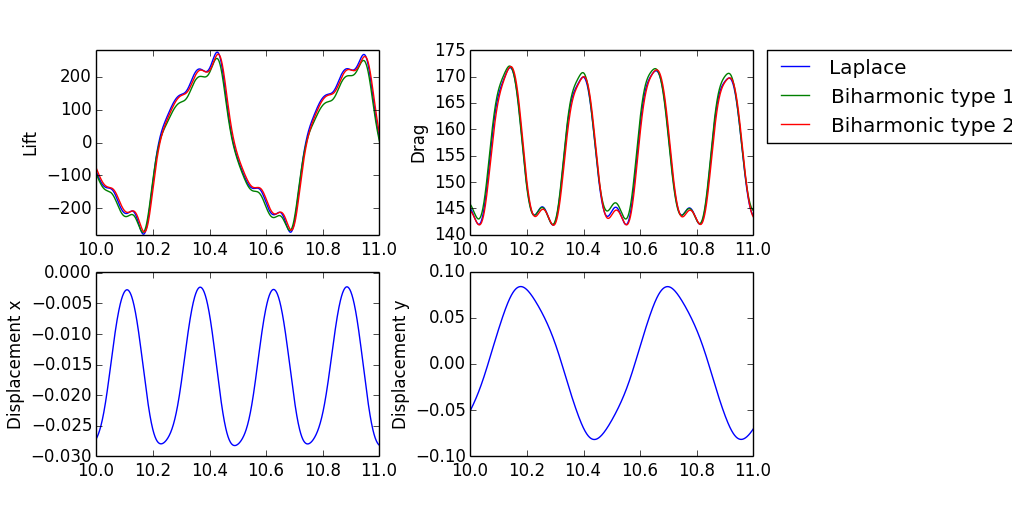
\includegraphics[scale=0.64]{./Fig/fsi2compare.png}
      \caption{FSI-2, visualization of fully developed flow with structure deformation at time t = 9s.}
\end{figure}
\begin{figure}[h!]
  \centering
    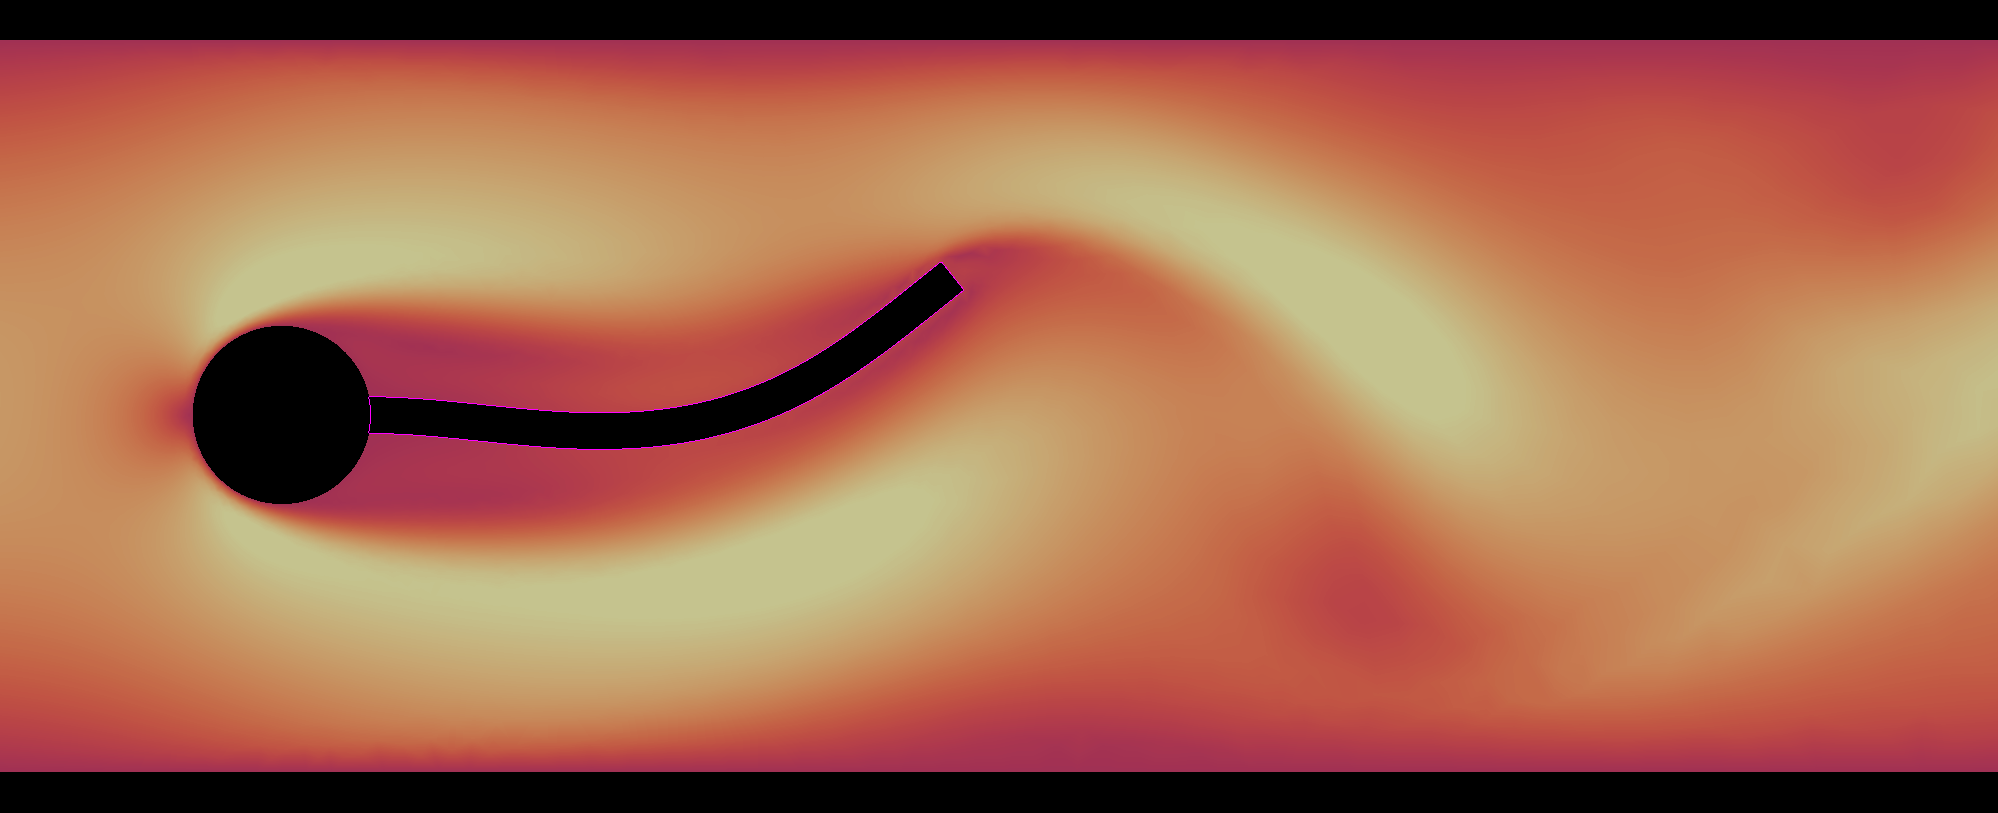
\includegraphics[scale=0.2]{./Fig/fsi2flow.png}
      \caption{FSI-2, visualization of fully developed flow with structure deformation at time t = 9s.}
\end{figure}
\newpage
\subsubsection{FSI-3}
\begin{table}[h!]
\centering
\caption{FSI 3 - Comparison of mesh extrapolation models}
\label{my-label}
\begin{tabular}{ |p{1cm}||p{1cm}|p{3.2cm}|p{3.2cm}|p{2.9cm}|p{3.1cm}|p{1.2cm}|}
 \hline
  \multicolumn{6}{|c|}{Laplace \hspace{2mm} $\Delta t = 0.01 \theta = 0.51$} \\
   \hline
nel & ndof & ux of A [x $10^{-3}$]  &uy of A [x $10^{-3}$]& Drag  & Lift \\
 \hline
 2474    & 21249  & -2.41 $\pm$   2.41 & 1.49     $\pm$   32.21 & 449.39       $\pm$   14.72 & 0.55 $\pm$   155.80  \\
 7307    & 63365  & -2.32    $\pm$   2.31 & 1.32 $\pm$    31.80 & 451.76  $\pm$   16.10 & 1.04      $\pm$   151.51  \\
 11556   & 99810  & -2.34  $\pm$   2.34  & 1.59   $\pm$  31.91 & 455.94       $\pm$ 17.34 & -0.01   $\pm$   151.36 \\
 \hline
  \multicolumn{6}{|c|}{$\Delta t = 0.001 \theta = 0.5$} \\
   \hline
 nel & ndof & ux of A [x $10^{-3}$]  &uy of A [x $10^{-3}$]& Drag  & Lift \\
    \hline
 2474    & 21249  & -2.91     $\pm$   2.74 & 1.28   $\pm$   35.01 & 450.90      $\pm$  18.11 & 2.28       $\pm$161.13 \\
 7307    & 63365  & -2.82    $\pm$   2.66& 1.24     $\pm$   34.69 & 453.56       $\pm$ 19.80 & 2.94     $\pm$ 158.67 \\
 11556   & 99810  & -2.88     $\pm$   2.72 & 1.49   $\pm$ 34.97 & 458.60   $\pm$ 22.12 & 2.23    $\pm$ 158.95 \\
 \hline
  \multicolumn{2}{|c|}{Reference} & -2.69 $\pm$  2.56                    & 1.48  $\pm$  34.38                   & 457.3  $\pm$  22.66        & 2.22  $\pm$ 149.78           \\
  \hline
    \multicolumn{2}{|c|}{Error}  & (7.0 $\pm$ 6.2)$10^{-6}$  \% & (6.7 $\pm$ 1.7)$10^{-6}$  \% & 0.28 \% $\pm$ 2.38 \% & 0.45 \% $\pm$ 6.12 \%\\
   \hline
\end{tabular}
\end{table}
\begin{table}[h!]
\centering
%\caption{FSI 3 - Biharmonic BC1}
\label{my-label}
\begin{tabular}{ |p{1cm}||p{1cm}|p{3.2cm}|p{3.2cm}|p{2.9cm}|p{3.1cm}|p{1.2cm}|}
 \hline
  \multicolumn{6}{|c|}{Biharmonic 1 \hspace{2mm}  $\Delta t = 0.01 \theta = 0.51$} \\
   \hline
nel & ndof & ux of A [x $10^{-3}$]  &uy of A [x $10^{-3}$]& Drag  & Lift \\
 \hline
 2474     &21249  & -2.40 $\pm$ 2.38  & 1.58 $\pm$ 32.07  & 450.16  $\pm$ 15.11  & -20.09 $\pm$ 148.17 \\
 7307    & 63365  &  -2.26 $\pm$ 2.14  & 1.70  $\pm$ 31.3 & 457.37  $\pm$ 15.24 & -51.77 $\pm$ 127.28 \\
 11556   & 99810  &   -2.33 $\pm$ 2.32 &  1.93   $\pm$ 31.5  & 456.40 $\pm$ 17.45 &  0.45 $\pm$ 149.68  \\
 \hline
  \multicolumn{6}{|c|}{$\Delta t = 0.001 \theta = 0.5$} \\
   \hline
 nel & ndof & ux of A [x $10^{-3}$]  &uy of A [x $10^{-3}$]& Drag  & Lift \\
 2474    & 21249  & -2.18 $\pm$ 2.10& 3.52 $\pm$ 2.90 & 435.19   $\pm$   9.77  & -1.59$\pm$   151.45 \\
 7307    & 63365  & -2.80 $\pm$ 2.64 & 1.25 $\pm$ 3.45 & 454.38   $\pm$   19.76 & 17.97  $\pm$  155.08 \\
 11556   & 99810  & -2.84 $\pm$ 2.68  & 1.50 $\pm$ 3.47 & 459.12    $\pm$   22.97 & -3.12     $\pm$ 171.22 \\
 \hline
 \multicolumn{2}{|c|}{Reference} & -2.69 $\pm$  2.56                    & 1.48  $\pm$  34.38                   & 457.3  $\pm$  22.66        & 2.22  $\pm$- 149.78           \\
 \hline
 \multicolumn{2}{|c|}{Error}  & (5.5 $\pm$ 4.6)$10^{-6}$ \% & (1.3 $\pm$ 8.9)$10^{-6}$ \%  & 0.40 \% $\pm$ 1.37 \% & 240.5 \% $\pm$ 14.3 \%\\
 \hline
\end{tabular}
\end{table}
\begin{table}[h!]
\centering
%\caption{FSI 3 - Biharmonic BC2}
\label{my-label}
\begin{tabular}{ |p{1cm}||p{1cm}|p{3.2cm}|p{3.2cm}|p{2.9cm}|p{3.1cm}|p{1.2cm}|}
 \hline
  \multicolumn{6}{|c|}{Biharmonic 2 \hspace{2mm}  $\Delta t = 0.01 \theta = 0.51$} \\
   \hline
nel & ndof & ux of A [x $10^{-3}$]  &uy of A [x $10^{-3}$]& Drag  & Lift \\
 \hline
 2474    & 21249  &-2.33 $\pm$ 2.33 & 1.57 $\pm$ 31.6    & 449.44  $\pm$ 14.82 & 0.80  $\pm$152.03  \\
 7307    & 63365  & -2.25 $\pm$ 2.23 &  1.35 $\pm$ 31.3  & 452.63     $\pm$16.29 & 17.11     $\pm$  146.05 \\
 11556   & 99810  & -2.25  $\pm$ 2.29 & 1.59  $\pm$ 31.4 & 457.89   $\pm$ 17.26 & 57.83      $\pm$  141.69 \\
 \hline
  \multicolumn{6}{|c|}{$\Delta t = 0.001 \theta = 0.5$} \\
   \hline
 nel & ndof & ux of A [x $10^{-3}$]  &uy of A [x $10^{-3}$]& Drag  & Lift \\
 2474    & 21249  & -2.83 $\pm$ 2.66   & 1.31 $\pm$ 34.5  &  450.24    $\pm$  18.25 & 2.57  $\pm$   175.42  \\
 7307    & 63365  & -2.77 $\pm$ 2.61    & 0.98$\pm$  34.6 & 453.53    $\pm$ 20.01 & 2.60   $\pm$ 159.13  \\
 11556   & 99810  & -2.80  $\pm$ 2.65 & 1.37 $\pm$ 34.7 & 458.41  $\pm$ 22.23 & 15.56   $\pm$  157.78 \\
 \hline
 \multicolumn{2}{|c|}{Reference} & -2.69 $\pm$  2.56                    & 1.48  $\pm$  34.38                   & 457.3  $\pm$  22.66        & 2.22  $\pm$- 149.78           \\
 \hline
 \multicolumn{2}{|c|}{Error}  & (4.0 $\pm$ 3.5)$10^{-6}$ \% & (7.4 $\pm$ 9.3)$10^{-6}$ \% & 0.24 \% $\pm$ 1.90 \% & 600.9 \% $\pm$ 5.34 \% \\
 \hline
\end{tabular}
\end{table}
\newpage
\begin{figure}[h!]
    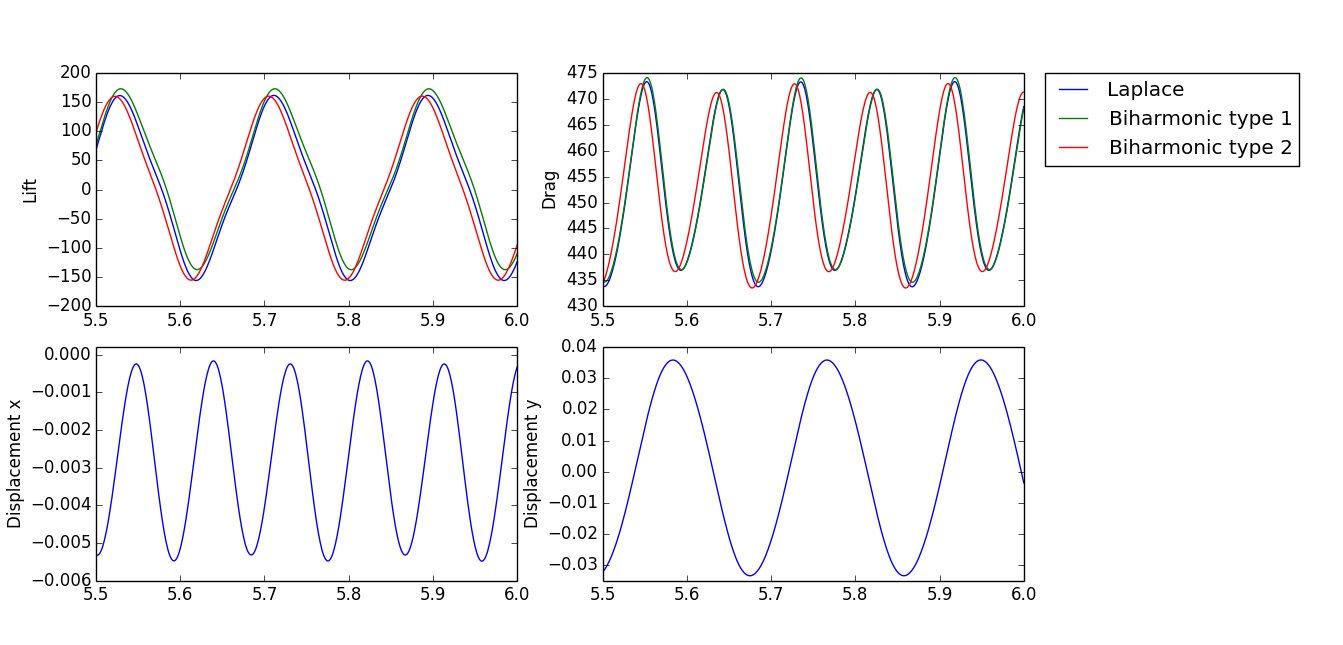
\includegraphics[scale=0.5]{./Fig/fsi3compare.png}
      \caption{Comparison of mesh motion models for FSI-3, in time interval t $t \in [5.5, 6]$.}
\end{figure}
\begin{figure}[h!]
  \centering
    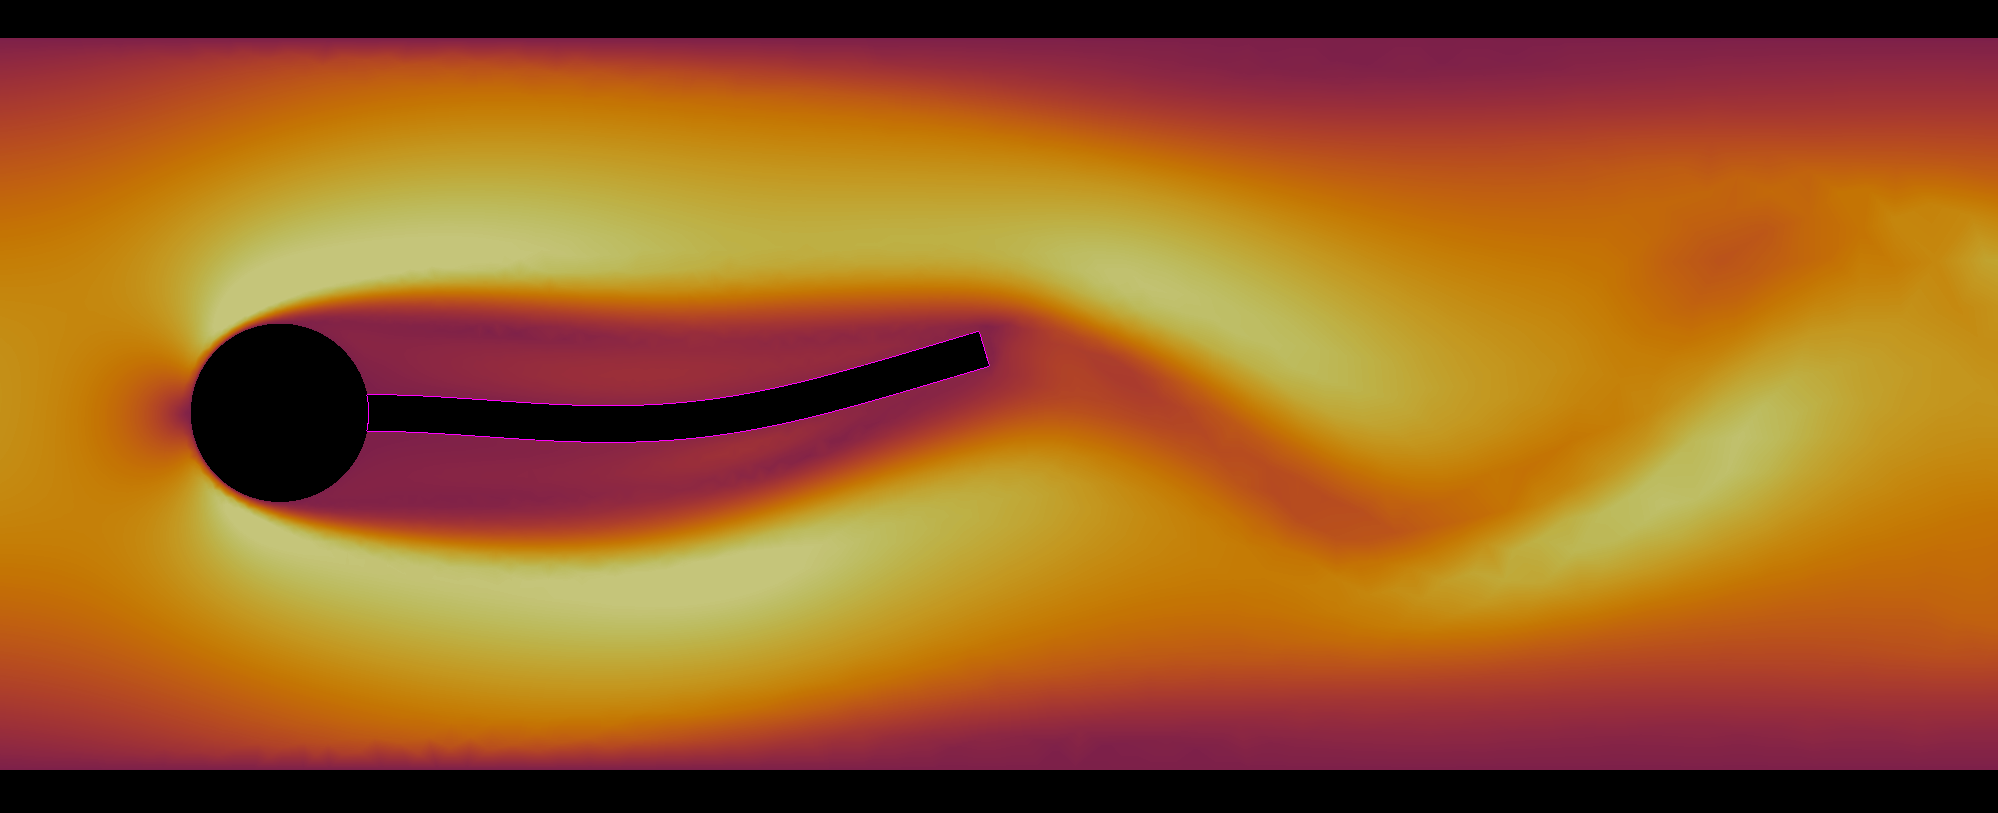
\includegraphics[scale=0.2]{./Fig/fsi3flow.png}
      \caption{FSI-3, visualization of fully developed flow with structure deformation at time t = 5.1s.}
\end{figure}
\newpage
\subsubsection*{Discussion}
For FSI-1, all models excel well in comparison with the reference solution, even at coarse mesh resolution. Due to low reynolds number flow the induced deformation of the elastic flag is very small, FSI-1 proves to be excellent for initial validation of fluid-structure interaction solvers. However, due the small deformations of the elastic flag of order $10^{-5}$,  FSI-1 doesn't provide a rigorous test case for mesh extrapolation models.  By omitting mesh extrapolation from the variational formulation in section 3.3.2,  reasonable results are still obtained in Table 4.10. This fact proves FSI-1 to be misleading in terms of mesh extrapolation model, but remains excellent for initial validation of fluid-structure interaction solvers and the overall coupling of the fluid and solid equations. \\
The FSI-2 problem proved to be one of the most demanding tests, due to the large deformation of the elastic flag. For large deformations, the chance of fluid mesh entanglement was considerably high, stressing the mesh lifting operator extensively. The linear elastic model failed for both time sizes, but not due to mesh entanglement but early failure of the Newton-solver. This finding is comparable with the investigation conducted in \cite{Richter2015}, where early failure of the Newton-solver is in context with long-term simulation of the implicit Crank-Nicolson scheme. In their study, a shifted implicit shifted Crank-Nicolson scheme $\theta = 0.5 + \Delta t$ proved to further improve stability for the newton-solver, making the numerical scheme stable for coarse time-step. Further, numerical investigation in \cite{Richter2015} showed that for both Crank-Nicolson and  shifted Crank-Nicolson are stable for $\Delta t < 0.003$ for the same benchmark. The numerical results in this thesis proved both implicit schemes was applicable for all mesh lifting operators, except the linear elastic model. \\
In general, the numerical solution regarding deformation of the elastic flag proved accurate in accordance with the reference solution for all sub-problems. However, the evaluation of drag and lift proved challenging for the periodic FSI-2 and FSI-3 problems. For FSI-2, poor accuracy was observed for all mesh resolutions and time steps, while for FSI-3 the evaluation of drag remained accurate. The same observations was found in \cite{Turek}, a followup work of the original benchmark \cite{Hron2006}, where numerical solutions committed by different research communities was compared. The diversity of lift and drag values provided by different research communities was surprising, as differences of order $50\%$ for drag and lift values, and $10\%$ for displacement was observed. More surprisingly was that the authors of the original benchmark \cite{Hron2006}, who also committed their numerical results, didn't match their own reference solution with the same solver. Therefore,  comparison of lift and drag forces with the reference solution alone can be misleading, and should not be the main acceptance criteria for code validation for this benchmark. Given the remarks in \cite{Turek}, the comparison of deformation is arguably a better main acceptance criteria. On this basis, the FSI code is validated in accordance with the original benchmark.  \\
 
%Validation of FSI is demanding due to the number of building blocks composing the full problem. For \textit{interface-tracking} methods such as the ALE-method, validation is not only related to the physical aspects of the model. Even if the fluid and structure models excel well within predefined criteria, the non-physical nature of mesh moving models have proven to affect the numerical solution \cite{Wickb}. At first glance, this effect is surprising as mesh moving models simply describe the evolution of fluid mesh cells from the moving interface. However, each model distributes %t'he fluid cells differently, which in turn may have an important effect when conducting mathematical operations such %as gradients. 
